% This is samplepaper.tex, a sample chapter demonstrating the
% LLNCS macro package for Springer Computer Science proceedings;
% Version 2.20 of 2017/10/04
%
\documentclass[conference]{IEEEtran}
\IEEEoverridecommandlockouts
%
\usepackage{cite}
\usepackage{amsmath,amssymb,amsfonts}
\usepackage{algorithmic}
\usepackage{graphicx}
\usepackage{textcomp}
\usepackage{xcolor}
% Used for displaying a sample figure. If possible, figure files should
% be included in EPS format.
%
% If you use the hyperref package, please uncomment the following line
% to display URLs in blue roman font according to Springer's eBook style:
% \renewcommand\UrlFont{\color{blue}\rmfamily}
\usepackage{hyperref}
\usepackage{caption}
\usepackage{subcaption}
\hypersetup{
    colorlinks=true,
    linkcolor=blue,
    filecolor=magenta,      
    urlcolor=cyan,
    }
\usepackage{tikz}
\usepackage{pgfplots}
\usetikzlibrary{positioning}
\usepackage{cleveref}
\usepackage{multirow}
\newcommand{\transform}[1]{\mathsf{T}(#1)}
\newcommand{\fitness}[1]{\mathsf{Fitness}(#1)}
\newcommand{\intensity}[1]{\mathsf{E}(#1)}
\newcommand{\edge}[1]{\mathsf{ne}(#1)}
\newcommand{\entropy}[1]{\mathsf{H}(#1)}
\usetikzlibrary{arrows.meta, positioning}
\def\BibTeX{{\rm B\kern-.05em{\sc i\kern-.025em b}\kern-.08em
    T\kern-.1667em\lower.7ex\hbox{E}\kern-.125emX}}

\begin{document}
%
% \title{Image Contrast Enhancement using Fuzzy Technique with Parameter Determination using Metaheuristics}

\title{Image Contrast Enhancement using Fuzzy Technique with Membership Function Determination using Metaheuristics}
%
%\titlerunning{Abbreviated paper title}
% If the paper title is too long for the running head, you can set
% an abbreviated paper title here
%
% \author{Mohimenul Kabir\inst{1} \and
% Jaiaid Mobin\inst{2} \and
%  Ahmad Hassanat\inst{3} \and 
% M. Sohel Rahman\inst{2}\thanks{Corresponding Author: \url{msrahman@cse.buet.ac.bd}}}
% %
% \authorrunning{Kabir et al.}
% \titlerunning{Image Contrast Enhancement}
% % First names are abbreviated in the running head.
% % If there are more than two authors, 'et al.' is used.
% %
% \institute{
% National University of Singapore
% \and
% Bangladesh University of Engineering \& Technology \and
% Mutah University}
%
\maketitle              % typeset the header of the contribution
%
\begin{abstract}
In this work, we have presented a way to increase the contrast of an image. Our target is to find a transformation that will be image-specific. We have used a fuzzy system as our transformation function. To tune the system according to an image, we have used the Genetic Algorithm and Hill Climbing in multiple ways to evolve the fuzzy system and conducted several experiments. Different variants of the method are tested on several images and two variants that are superior to others in terms of fitness are selected. We have also conducted a survey to assess the visual improvement of the enhancements made by the two variants. The survey indicates that one of the methods can enhance the contrast of the images visually.
\end{abstract}

\begin{IEEEkeywords}
image enhancement, metaheuristics,  fuzzy logic, genetic algorithm
\end{IEEEkeywords}
%
%
%
\section{Introduction}
Image enhancement is the process of improving an image's quality and information content~\cite{singh2014various}. The goal is to increase visual differences among image features, making it more suitable for various applications, such as increasing the brightness of dark images for better viewing. Common image enhancement techniques include sharpening, smoothing, contrast enhancement, and noise reduction~\cite{draa2014artificial}. Contrast enhancement, in particular, is applied to images or videos to increase their dynamic range~\cite{hashemi2010image}.

Image enhancement has been practiced as an applicable problem in meta-heuristics for a long time~\cite{cuckoo_search_and_PSO,ACO_GA_SA,munteanu2004gray,mukhopadhyay2023image}. Moreover, the integration of fuzzy systems with meta-heuristic algorithms has been the subject of area within the Computational Intelligence 
community~\cite{fuzzy_plus_meta,diaz2017new}. Many studies have approached image enhancement as an optimization problem, focusing on modifying the image quality fitness function~\cite{cuckoo_search_and_PSO,draa2014artificial,oloyede2019new}, combining several meta-heuristic algorithms~\cite{cuckoo_search_and_PSO,ACO_GA_SA}, optimizing parameters \cite{samanta2018log} and avoiding local optima \cite{dos2009differential}. However, one aspect that has not received as much attention in image enhancement problems is the adaptation of fuzzy systems. Sandeep and Samrudh~\cite{s2018image} have demonstrated that the variation in the input membership function in a fuzzy system can positively impact image enhancement performance.

This paper addresses the image contrast enhancement problem by using stochastic optimization within a fuzzy logic system. 
Our primary contribution is the design of a meta-heuristic inspired framework that leverages a fuzzy logic system.
The core component of the fuzzy logic system is a set of {\em input membership function} that are used to describe an {\em intensity transformation function}. 
We implement genetic operators that {\em mutate} the fuzzy logic system, thereby enhancing the original image to achieve optimal contrast enhancement. 
The fuzzy system in our approach is based on simple contrast enhancement rules, outlined in \cite{gonzalez2008digital}, and it operates independently of the input image.

Our main idea of the fuzzy image enhancement technique is as follows: we start with a basic fuzzy rule set and a set of input membership functions. By applying a metaheuristics framework, we try to evolve the fuzzy sets. Finally, we apply the transformation function described by fuzzy sets on the value channel of HSV color space to get the final image. Thus we have converted the problem into an optimization problem. In other words, rather than generating an image, we try to generate a suitable mapping between the input and output color values. However, this is inherently challenging since, even if we consider only 8-bit color, i.e., $256$ color values, the number of possible mappings becomes huge. Thus it becomes infeasible to search through the solution space exhaustively, and there is no definite knowledge about how to improve/generate a solution. This motivates us to leverage a metaheuristics framework \cite{Luke2009Metaheuristics}.
\section{Literature Review}
\label{section:literature}
Several techniques are used for contrast manipulation, including gamma transformation~\cite{singh2014various} and histogram equalization (HE)~\cite{singh2015histogram,stark2000adaptive}, but it has limitations, such as failing to maintain image brightness~\cite{shanmugavadivu2014particle}. Bi-histogram Equalization~\cite{ooi2009bi} addresses this issue. Another drawback of HE is the potential loss of image information~\cite{zhu2012adaptive}. Techniques like gamma transform and log transform~\cite{singh2014various} offer lower computational complexity. Tarawneh et al.~\cite{tarawneh2020automatic} applied gamma transformation for contrast enhancement by automatically applying different gamma corrections to multiple pixel sets. However, these techniques often struggle in complex illumination settings~\cite{oloyede2019new}, requiring parameter adjustments to be effective.
Bhandari et al~\cite{bhandari2019novel} combined sub-histograms with {\em discrete cosine transform} for contrast enhancement.

Fuzzy logic and metaheuristic techniques have been previously applied to image enhancement problems~\cite{korytkowski2020efficient,fuzzy_plus_meta,diaz2017new}. A fundamental approach involves using a fuzzy logic-based system from \cite{gonzalez2008digital}, which utilizes only three rules and employs trapezoidal and triangular input fuzzy sets. In contrast, Joshi and Kumar~\cite{s2018image} proposed a more complex method with a seven-rule set and Gaussian fuzzy sets.

To evaluate the fitness of an enhanced image, Munteanu and Rosa~\cite{munteanu2004gray} proposed a novel objective function and applied an evolutionary algorithm to search for optimal parameters in a continuous transform function. This objective function has also been utilized in various optimization techniques, including artificial bee colony optimization~\cite{draa2014artificial}, the cuckoo search algorithm~\cite{bhandari2020cuckoo}, and the firefly algorithm for enhancing UAV-captured images~\cite{samanta2018log}.
\iffalse
From this brief review, we can see that both the metaheuristics framework and the fuzzy logic system is a used approach in image enhancement. The limitation of current fuzzy logic-based literature is that the fuzzy logic systems used are constant logic systems. Using the metaheuristics framework, deriving a better fuzzy logic system for image enhancement can be automated.
\fi
\section{Preliminaries}
\subsection*{Fuzzy Image Processing}
Fuzzy image processing encompasses a range of techniques designed to understand, represent, and process images, along with their segments and features, as {\em fuzzy sets} (see Figure \ref{fig:fii}). The process begins with the {\em fuzzification} (or encoding) of image data, followed by the {\em defuzzification} (or decoding) of the results. These steps enable the application of fuzzy techniques to image processing. At the core of fuzzy image processing lies {\em membership modification}~\cite{haussecker2000fuzzy}. The workflow of fuzzy image processing is illustrated in~\Cref{fig:fii}.

\begin{figure*}
    \centering
    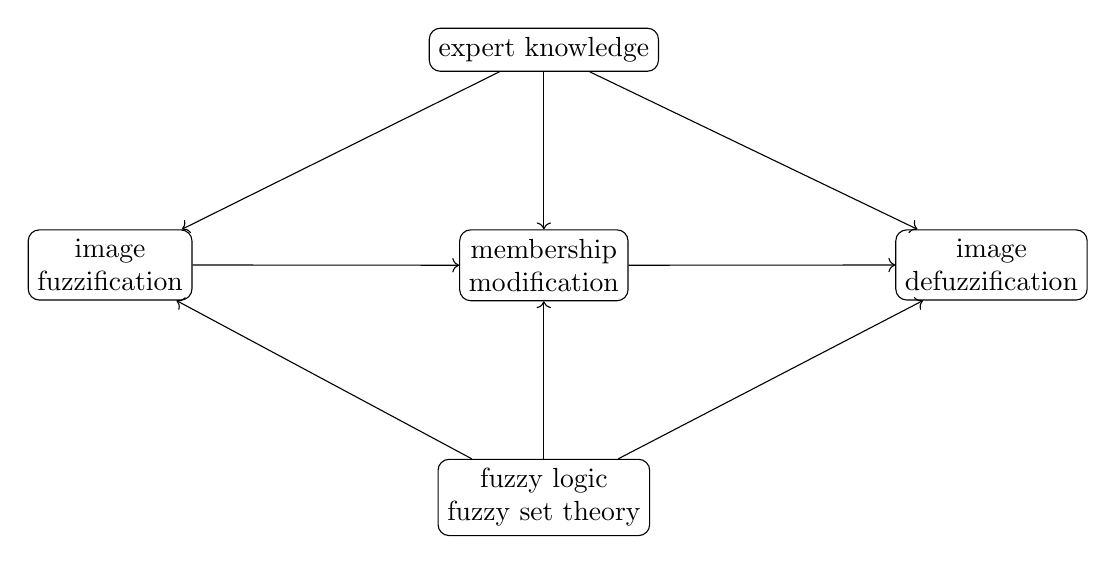
\begin{tikzpicture}[
        node distance=2cm and 3cm,
        every node/.style={draw, align=center, rounded corners},
        every edge/.style={draw, -{Latex[length=3mm]}}
    ]
    
    % Nodes
    \node (expert) {expert knowledge};
    \node (fuzzification) [below left=of expert] {image\\ fuzzification};
    \node (modification) [below=of expert] {membership\\ modification};
    \node (defuzzification) [below right=of expert] {image\\ defuzzification};
    \node (fuzzy) [below=of modification] {fuzzy logic \\ fuzzy set theory};
    
    % Edges
    \draw[->] (expert) -- (fuzzification);
    \draw[->] (expert) -- (modification);
    \draw[->] (expert) -- (defuzzification);
    \draw[->] (fuzzification) -- (modification);
    \draw[->] (modification) -- (defuzzification);
    \draw[->] (fuzzy) -- (fuzzification);
    \draw[->] (fuzzy) -- (modification);
    \draw[->] (fuzzy) -- (defuzzification);
    \end{tikzpicture}
    \caption{The workflow of fuzzy image processing}
    \label{fig:fii}
\end{figure*}
\subsection*{Fuzzy Sets for Intensity Transformation}
Contrast enhancement is one of the principal
applications of intensity transformations. We can state the process of enhancing the contrast of a gray-scale image using the following rules \cite{gonzalez2008digital}:
\begin{itemize}
    \item IF a pixel is \textbf{dark}, THEN make it \textbf{darker}
    \item IF a pixel is \textbf{gray}, THEN make it \textbf{gray}
    \item IF a pixel is \textbf{bright}, THEN make it \textbf{brighter}
\end{itemize}
\section{Problem Statement}
\label{section:problem}
Our objective is to manipulate image contrast to enhance the sharpness and make image features more visually distinguishable. While image enhancement is inherently subjective, we have employed a fitness function from image enhancement literature to quantify this enhancement \cite{bhandari2020cuckoo,draa2014artificial,dos2009differential,braik2007particle,munteanu2004gray}. This fitness function evaluates the quality of an enhanced image. We use a transformation function to enhance the image, which is optimized using a metaheuristic approach. Thus, the input to our process is an image, and the output is an enhanced version of that image.

For simplicity, we present a formal definition of the problem in the context of a {\em grayscale} image. Let $I = f(x, y)$ represent a grayscale image, where $x$ and $y$ denote the pixel positions. The image $I$ has dimensions $M \times N$, thus $0 \leq x < M$ and $0 \leq y < N$. Assume there is a fuzzy logic-based transformation function $\transform{I}$ that modifies the gray value of each pixel, producing an enhanced image $I_e$. More formally,


% We give a more formal definition of the problem below in the context of a gray-scale image (for simplicity). Suppose a gray-scale image, $I = f(x,y)$, where $x$ and $y$ denote the pixel's positions of the image. Let the image $I$ have a dimension of $M \times N$. So,  $0\leq x < M$ and $0\leq y < N$. Now assume that there is a fuzzy logic-based transformation function $\transform{I}$ that transforms the gray value of each pixel of the image and outputs another image or enhanced image $I_e$. More formally,
\begin{equation} \label{eqn:transformation}
I_e = \transform{I} = \transform{f(x,y)}
\end{equation}
Thus, our task is to identify a suitable transformation function that visually enhances the resulting image $I_e$.










\section{Methodology}
\label{section:method}
In this section, we present our meta-heuristic-based methodology for image contrast enhancement. Meta-heuristic methods share several common features~\cite{glover2003handbook}. Each method begins with an initial set of {\em individuals}, often referred to as the {\em population}. To introduce diversity into the population, special operations, known as {\em mutations}, are applied to generate new populations. In each iteration, the fittest individuals are selected based on a mathematical function known as the {\em fitness function}. This process of generating new population is repeated for a fixed number of iterations, with the fittest population from all iterations is considered the best solution found. While this approach does not guarantee an optimal solution, it is effective at discovering {\em good} solutions within a relatively short time frame. However, the difference between most meta-heuristics algorithms lies in the way in which the initial population is generated and the mutation function is applied. 

At a high level, we employed Hill Climbing and Genetic Algorithm-based techniques, exploring five different variants of these approaches. Specifically, we implemented three variants of Hill Climbing and two variants of the Genetic Algorithm. For the Hill Climbing approach, the variants differ in their mutation functions and input membership functions, as detailed below. For the Genetic Algorithm, we used a single type of input membership function, with variations in the next generation selection strategies (see Section \ref{subsection:method_ga_join}).
% \begin{itemize}
%     \item Hill Climbing
%         \begin{enumerate}
%             \item neighborhood generation using simple mutation
%             \item neighborhood generation with Trapezoidal and triangular input membership set splitting mutation
%             \item mixed neighborhood generation with Gaussian input membership set splitting mutation
%         \end{enumerate}
%     \item Genetic Algorithm
%     \begin{enumerate}
%             \item simple neighborhood generation with Trapezoidal and Triangular input membership set
%             \item simple neighborhood generation with Gaussian and Sigmoid input membership set
%         \end{enumerate}
% \end{itemize}
First, we discuss the subroutines that are common among all variants of metaheuristics approaches, namely, initialization, representation, and fitness assessment. 
\begin{figure}
    \centering
    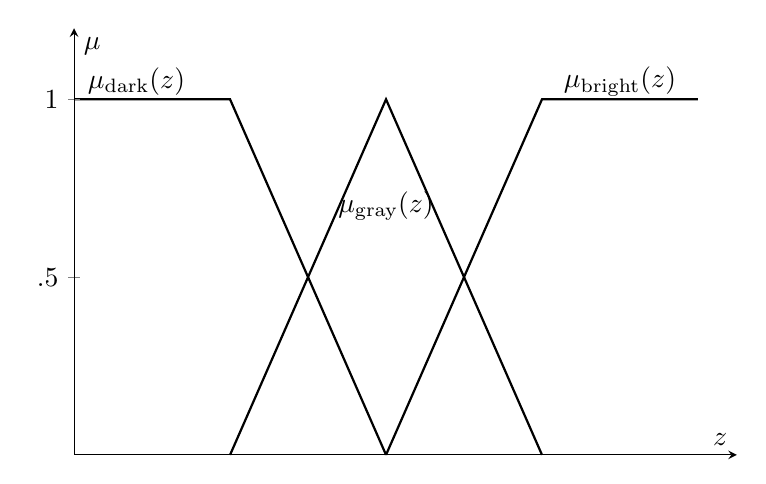
\begin{tikzpicture}
        \begin{axis}[
            axis lines=middle,
            xlabel={$z$},
            ylabel={$\mu$},
            ymin=0, ymax=1.2,
            xmin=0.0, xmax=8.5,
            xtick=\empty,
            ytick={0, 0.5, 1},
            yticklabels={0, .5, 1},
            width=10cm,
            height=7cm,
            enlargelimits=false,
            axis on top,
            clip=false,
            domain=-1:8
            ]
    
            % Dark membership function
            \addplot[thick] coordinates {(0,1) (2,1) (4,0)};
    
            % Gray membership function
            \addplot[thick] coordinates {(2,0) (4,1) (6,0)};
    
            % Bright membership function
            \addplot[thick] coordinates {(4,0) (6,1) (8,1)};
    
            % Labels
            \node at (axis cs: 0.8, 1.05) {$\mu_{\text{dark}}(z)$};
            \node at (axis cs: 4, 0.7) {$\mu_{\text{gray}}(z)$};
            \node at (axis cs: 7, 1.05) {$\mu_{\text{bright}}(z)$};
    
        \end{axis}
    \end{tikzpicture}
    \caption{Input membership functions for fuzzy, rule-based contrast enhancement  \cite{gonzalez2008digital}}
    \label{fig:fuzzy_function}
\end{figure}
% \begin{figure}
%     \centering
%     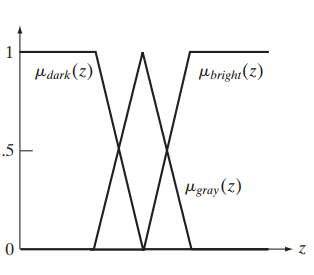
\includegraphics[scale=0.8]{fuzzy_function.PNG}

% \end{figure}


%\subsection*{Population Initialization}
\subsection{Population Representation}
\label{subsection:method_pop}
Every meta-heuristics technique starts with some (usually randomly generated) initial population and the structure of the population is specific to the problem we are aiming to solve. In our case, each candidate is an input membership function, as shown in Figure \ref{fig:fuzzy_function}. So, our population representation holds information about a set of input membership functions. Within each input membership function, there are at least three functions. Each membership function is represented by a tuple of three values regardless of the function types (i.e., trapezoidal, triangular, Gaussian, and Sigmoidal). The first two values of the tuple determine the shape of the membership function, and the third one is used in defuzzification.

\subsection{Fitness Assessment}
\label{subsection:fitness_assessment}
Following the literature of image enhancement~\cite{munteanu2004gray}, we calculate an individual's ($I$) quality/fitness using the following fitness function: 
%There are some terms in Equation \ref{eqn:fitness} which we will explain now, 
\begin{equation} \label{eqn:fitness}
\fitness{I} = \log{\log{\intensity{I_s}}} \times \frac{\edge{I_s}}{M \times N} \times \entropy{I_s}
\end{equation}
\begin{description}
    \item[$I_s$] $=$ image after Applying {\em Sobel filter} on $I$
    \item[$\intensity{I}$] $=$ sum of intensity of image $I$
    \item[$\edge{I}$] $=$ number of edge pixel in $I$
    \item[$\entropy{I}$] $=$ entropy of image $I$
    \item[$M$] $=$ width of $I$
    \item[$N$] $=$ height of $I$
\end{description}

\subsection*{HSV Conversion}
\label{subsection:method_hsv}
If the input image is a color image, we need to convert it to the HSV format. In the case of a gray-scale image, there is no need for such a conversion. 

\subsection*{Defuzzification}
\label{subsection:method_defuzz}
Defuzzification refers to converting the fuzzy value to a {\em single crisp} value. For any given input pixel $z_0$, the output crisp value $v_0$ will be as follows.
\begin{equation} \label{eqn:defuzzy}
v_0 = \frac{\sum\limits_{i=1}^n\mu_{i}(z_0) * v}{\sum\limits_{i=1}^n\mu_{i}(z_0)};n\geq3
\end{equation}
Here,
\begin{description}
    \item[$\mu_{i}(z_0) = $] \quad fuzzy level of the image pixel with value $z_0$
    \item[$v =$] constant/mutable value (depending on the algorithm variant) used in the defuzzification 
\end{description}

\subsection{Hill Climbing}
\label{subsection:method_hc}
The Hill Climbing technique stochastically generates new individuals and stores the fittest individual as the candidate solution. The best solution is evaluated using the fitness function shown in Equation \ref{eqn:fitness}. In each generation, we generate a certain number of neighbor solutions (set to $10$) from a fixed individual. We have tried three variants of Hill Climbing differing from each other in neighborhood generation and input membership function type.

\subsubsection{Simple Neighborhood Generation}
\label{subsubsec:simple_neighbour_generation}
In this variant, we have initiated an individual with two trapezoidal ($\mu\_dark, \mu\_bright$) and one triangular ($\mu\_gray$) functions like Figure \ref{fig:fuzzy_function}. 
When generating a new individuals, only the shapes of the functions (i.e., the width of the triangle and trapezoid's oblique line's slope) are tweaked. 
We have adapted three hyperparameters, namely, $\mathsf{ChangeProb}$, $\mathsf{MutateMu}$, and $\mathsf{MutateSigma}$. 
Firstly, $\mathsf{ChangeProb}$ represents the threshold of the random number chosen to decide whether the shape change will be performed or not. 
On the other hand, $\mathsf{MutateMu}$ and $\mathsf{MutateSigma}$ represent, respectively, the mean and variance of Gaussian distribution from which the random number is chosen when generating a new solution. 
% no need ===
% \subsubsection*{Neighborhood Generation with trapezoidal and triangular input membership set splitting mutation}
% \label{subsubsection:method_hc_traptri_split}
% This variant considers an additional tweak besides the previous one. A membership function may split into two membership functions (e.g., one triangle in Figure \ref{fig:fuzzy_function} splits into two). In addition to the previously mentioned parameters, here we have used another one, which is $\mathsf{MembershipSplitProb}$, to control the probability of choosing function shape change or input member function splitting.
% \subsubsection*{Neighborhood Generation with Gaussian input membership set splitting mutation}
% \label{subsubsection:method_hc_gauss_split}
% In this case, we have used only the Gaussian input membership function in our solution. All the hyperparameters mentioned in the previous two cases are used.

\subsection{Genetic Algorithm}
\label{subsection:method_ga}
Unlike Hill Climbing, the Genetic Algorithm (GA) starts with a number (say, $\mathsf{PopSize}$) of individuals. We use the same evaluation function shown in Equation \ref{eqn:fitness} for fitness evaluation in our GA approach. To introduce variations in the population, GA breeds a new population of children, selects individuals from the old population, and tweaks them to breed new individuals. To keep the footprints of both populations, it joins the parent and children populations to form a new generation of population. In our implementation, we have fixed $\mathsf{PopSize}$ equal to $30$.

\subsection{Tweaking Operations}
\label{subsection:method_ga_tweak}
\subsubsection{Crossover}
The crossover operation mixes multiple individuals (typically $2$) and matches to form the children. There are $3$ classical ways of doing a crossover. In our implementation, we have used {\em uniform crossover}. In the context of our representation, our crossover operation marches down all the membership functions and to combine them swaps individual functions if a coin toss comes up head with probability $p$. To use crossover on the Genetic Algorithm, both individuals should be of the same size. 

\subsubsection{Mutation}
\label{subsection:method_ga_mut}
Our mutation operation scans each membership function and randomly tweaks the function shape with a certain probability. To exploit both exploitation and exploration, our mutation operation uses a Gaussian distribution with a certain mean and variance. 
% Unlike Hill Climbing, mutation operation here does not increase/decrease the number of membership functions.

\subsection{Joining}
\label{subsection:method_ga_join}
The Genetic Algorithm differs in how parent and child populations are joined. In our Genetic Algorithm procedure, we have experimented with both $(P, P)$ and $(P+P)$ evolution strategies, where $P$ is the $\mathsf{PopSize}$.

% \subsection{Experiment Process}
% \label{subsection:experiment_process}
% In the experimental analysis, first, we choose the best variants among all variants of Hill Climbing and the Genetic Algorithm. Then we measure the performance of our image enhancement method with respect to common metrics of image enhancements, and finally, we compare our results with one of the simplest methods of image enhancement --- histogram equalization.
% %The objective of our experiment is first select the best two variants from the five variants we have experimented on, then we have measured different metrics of the output images to compare them with a simple contrast enhancement approach called histogram equalization.

% \subsubsection{Variant Selection}
% The following steps are used to choose the best variants:

% \begin{enumerate}
%     \item Run one variant on each image. The variant is applied on one image a total of $\mathsf{NumofTest}$ times. Each time (one stochastic optimization) is run for $ \mathsf{PerRunTime}$ seconds. This time is kept the same for all variants. Also, mutation and population initialization-related parameters are kept the same for all variants. 
%     %(except $SPLIT\_PROB$ because variants are also differentiated based on this).  
    
%     \item Measure the average rate of fitness improvement over the number of generations achieved in given $\mathsf{PerRunTime}$. Then the average is computed for $\mathsf{NumofTest}$ times.
    
%     \item We have compared the metric achieved in step $2$ for all five variants and then selected the best two variants. The higher the value of this metric demonstrates better performance.
% \end{enumerate}

The value of experiment controlling parameters is written in Table \ref{tab:exp_parameters}.

\begin{table}[]
    \centering
    \begin{tabular}{| c | c |}
        \hline
        \textbf{Hyperparameter name} & \textbf{Value}\\
        \hline
        $\mathsf{NumofTest}$ & $5$ \\ 
        \hline
        $\mathsf{PerRunTime}$ & $120$ \\
        \hline
        $\mathsf{ChangeProb}$ &  $0.5$\\
        \hline
        $\mathsf{MutateMu}$ & $3$ \\
        \hline
        $\mathsf{MutateSigma}$ & $2$ \\
        \hline
        $\mathsf{MembershipSplitProb}$ & $0.1$ \\
        \hline
    \end{tabular}
    \caption{The value of hyperparameters}
    \label{tab:exp_parameters}
\end{table}

 








 \section{Experimental Results}
In this section, we evaluate our proposed approach and present the results of applying our method to various images. Our experiments were conducted on several images from \cite{draa2014artificial} and additional images (color, grayscale, and text) sourced from the Internet. Specifically, we experimented with a total of 18 images.

\subsection{Experimental Setup and Environment}
To evaluate the efficacy of our approach, we implemented a prototype in Python using the DEAP evolutionary computation framework\footnote{\url{https://deap.readthedocs.io/en/master/}}. For the fuzzy logic component, we utilized the scikit-fuzzy toolbox\footnote{\url{https://pythonhosted.org/scikit-fuzzy/}}.

All variants of our algorithms were executed on a system with an Intel(R) Core(TM) i$3$ CPU M$370$ @ $2.40$GHz processor, $6$GB RAM, running Ubuntu $18.04$, and Python version $3.6.8$.
% will be available after acceptance
% Our experiment code can be found in this link, \href{https://dicta2024.dictaconference.org/}{redacted for review version}.

\subsection{Results}
\label{subsection:exp_result_result}

Here, we visually present outputs for a limited number of images due to our page limitation. Figures \ref{fig:07_output_image_hc}, \ref{fig:jetplane_output_image_hc}, \ref{fig:07_output_image_ga}, \ref{fig:house_output_image_ga} show output images generated by our technique against the reference input images.
As an outcome of our technique, the enhanced images are more clear and natural (Figures~\ref{fig:07_output_image_hc}, \ref{fig:07_output_image_ga}, \ref{fig:house_output_image_ga}), the edges are sharper (Figures \ref{fig:jetplane_output_image_hc},
\ref{fig:house_output_image_ga}), the histogram is expanded, and the contrast between black and white portion is increased. On the contrary, some black portions (Figures \ref{fig:jetplane_output_image_hc}, \ref{fig:07_output_image_ga}) are unnecessarily darkened. 

\subsection{Survey}
\label{subsection:exp_result_survey}
\subsubsection{Variant Selection to Select Survey Images}
First, we have grouped the variants according to used metaheuristic algorithms, namely Hill Climbing and Genetic algorithm. Then according to the method described in Subsection \ref{subsection:experiment_process}, we have ranked the variants among two groups. Based on this the selected variants from the two groups are as follows:
\begin{enumerate}
    \item (Method $1$) Hill Climbing with simple neighborhood generation (Subsection \ref{subsubsec:simple_neighbour_generation})
    \item (Method $2$) Genetic Algorithm with (P, P) strategy (Subsection \ref{subsection:method_ga_join})
\end{enumerate}

\subsubsection{Survey Preparation}
We have prepared an anonymous survey %\footnote{\url{https://forms.gle/9wuLKMYBShjyAaK59}} 
to get a quantitative opinion on our enhanced images. In the survey, we have placed $36$ enhanced images (produced by our technique) side-by-side with their original image. The first $18$ images are from Hill Climbing with neighborhood generation with split mutation (see Section \ref{subsubsection:method_hc_traptri_split}), and the second $18$ images are the same but from the Genetic Algorithm with (P, P) strategy (see Section \ref{subsection:method_ga_join}). The survey participant needs to mark the enhanced image on a scale of $1-9$. As the reference, the mark of the original image was $5$; therefore, a mark of $>5$ by the reviewer would mean an enhanced image, while $<5$ will mean image degradation. A mark of $5$ would mean the processed image is the same as the original visually (a subjective judgment). The prepared survey form can be found at the following link: \href{https://dicta2024.dictaconference.org}{redacted for review version}%\url{https://forms.gle/9wuLKMYBShjyAaK59}.
%\href{https://forms.gle/9wuLKMYBShjyAaK59}{here}.

\subsubsection{Survey Response \& Observations}
We have received a total of $67$ responses. From the responses, we have filtered responses with suspicious patterns like all equal marks or very high or very low marks. This filtering caused two responses to be filtered. From the remaining $65$ responses, it seems method $2$, achieving a mean score of $5.45$, is better than method $1$, achieving a mean score $4.77$. 
Moreover, achieving a mean score of greater that $5$ indicates that the method $2$ improves the original image.

\begin{figure}[!htb]
\begin{subfigure}{0.5\textwidth}%
  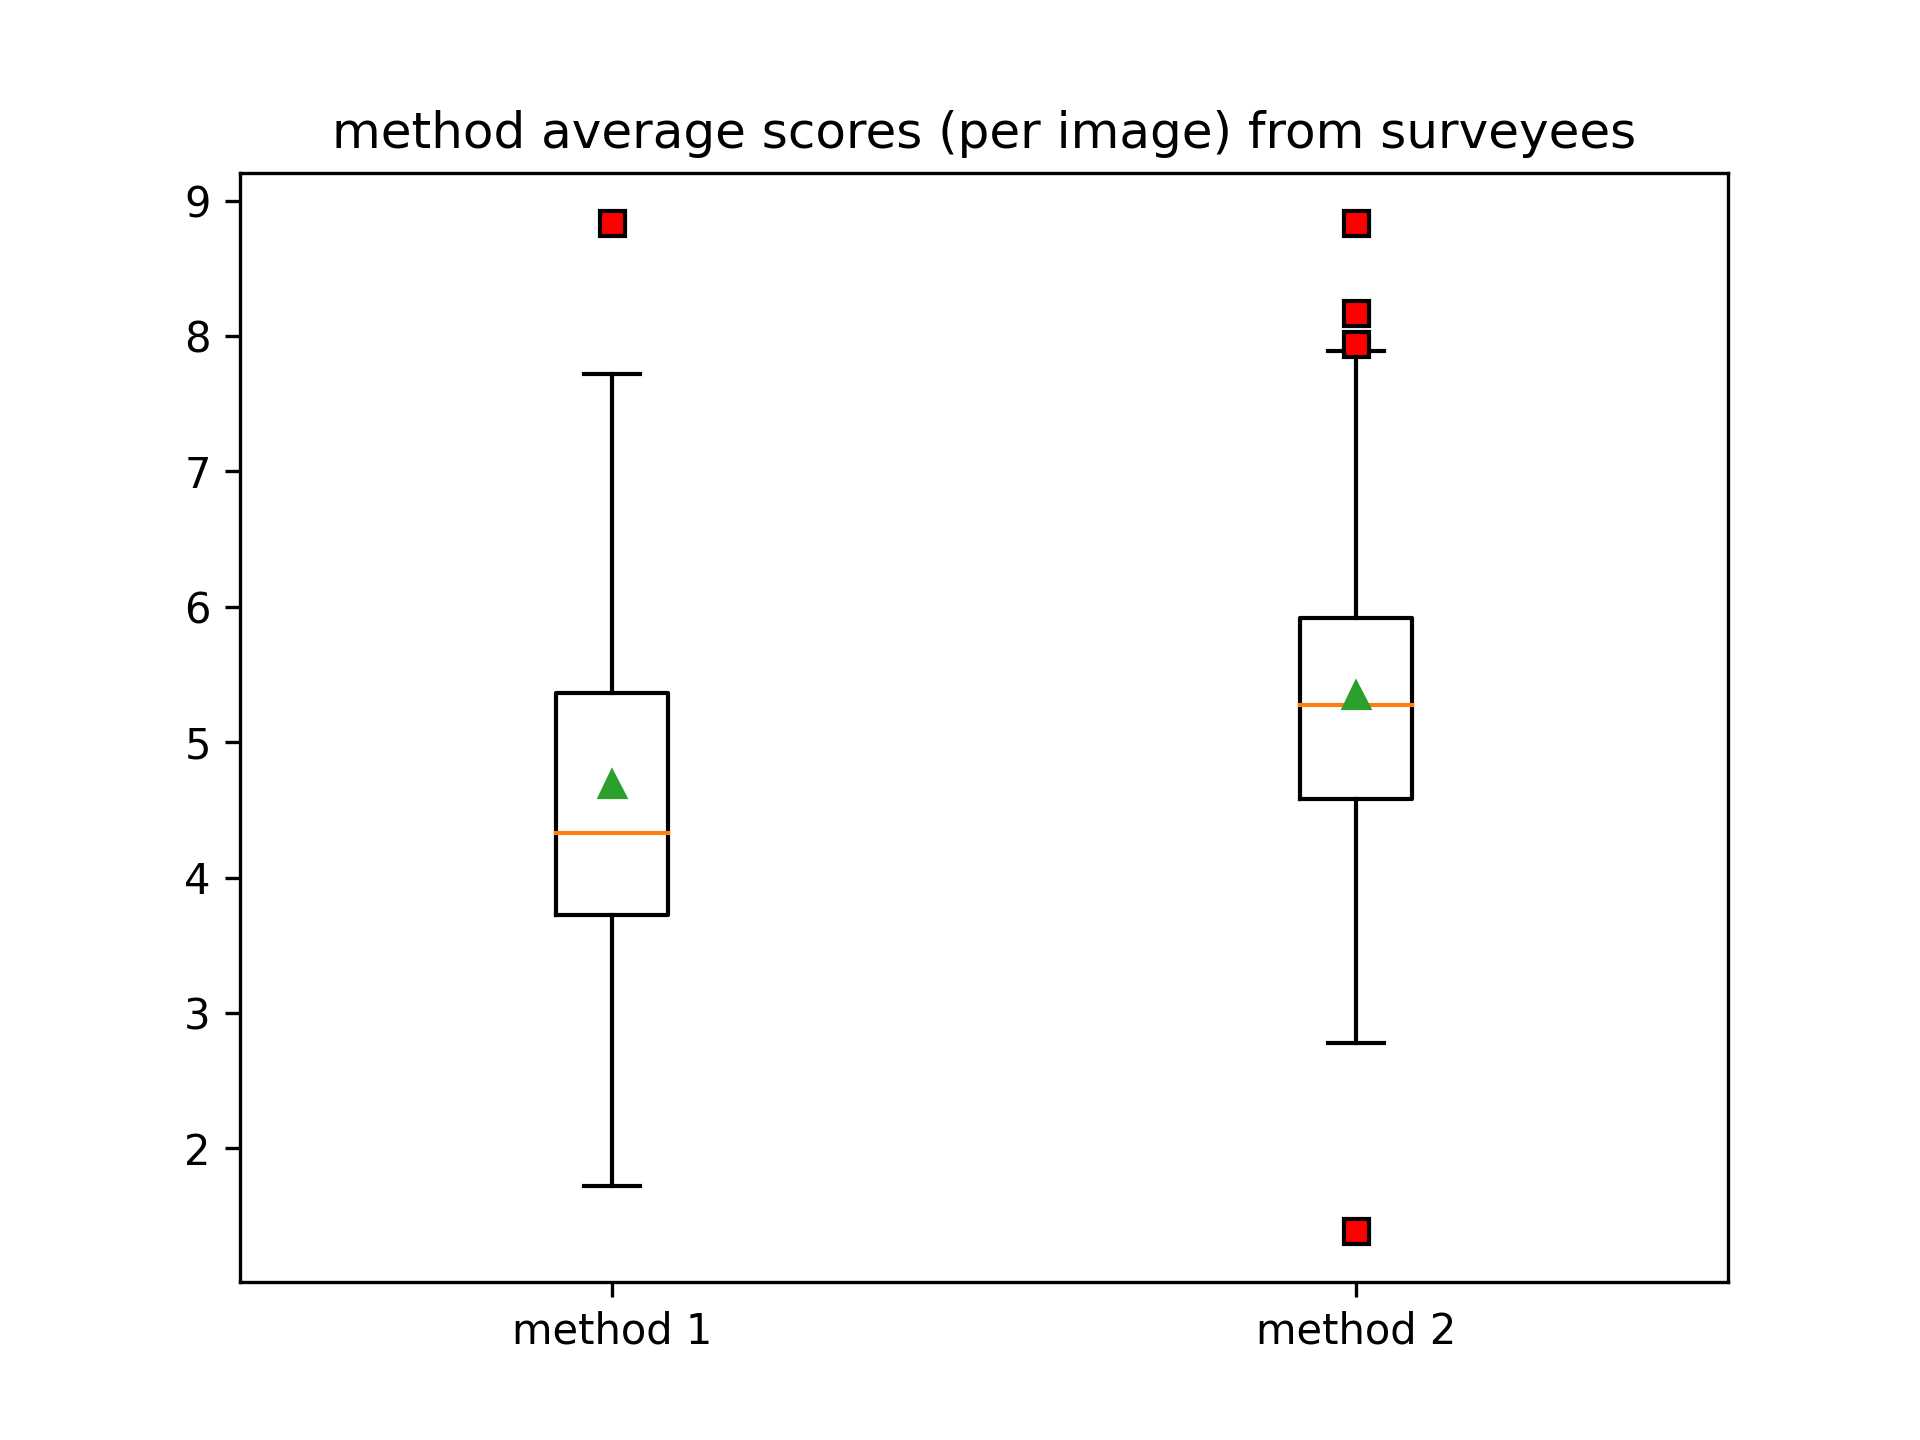
\includegraphics[width=\linewidth]{surveyee_score_box_plot.png}
  \caption{}
  \label{fig:survey_result_boxplot}
\end{subfigure}
\begin{subfigure}{0.5\textwidth}%
  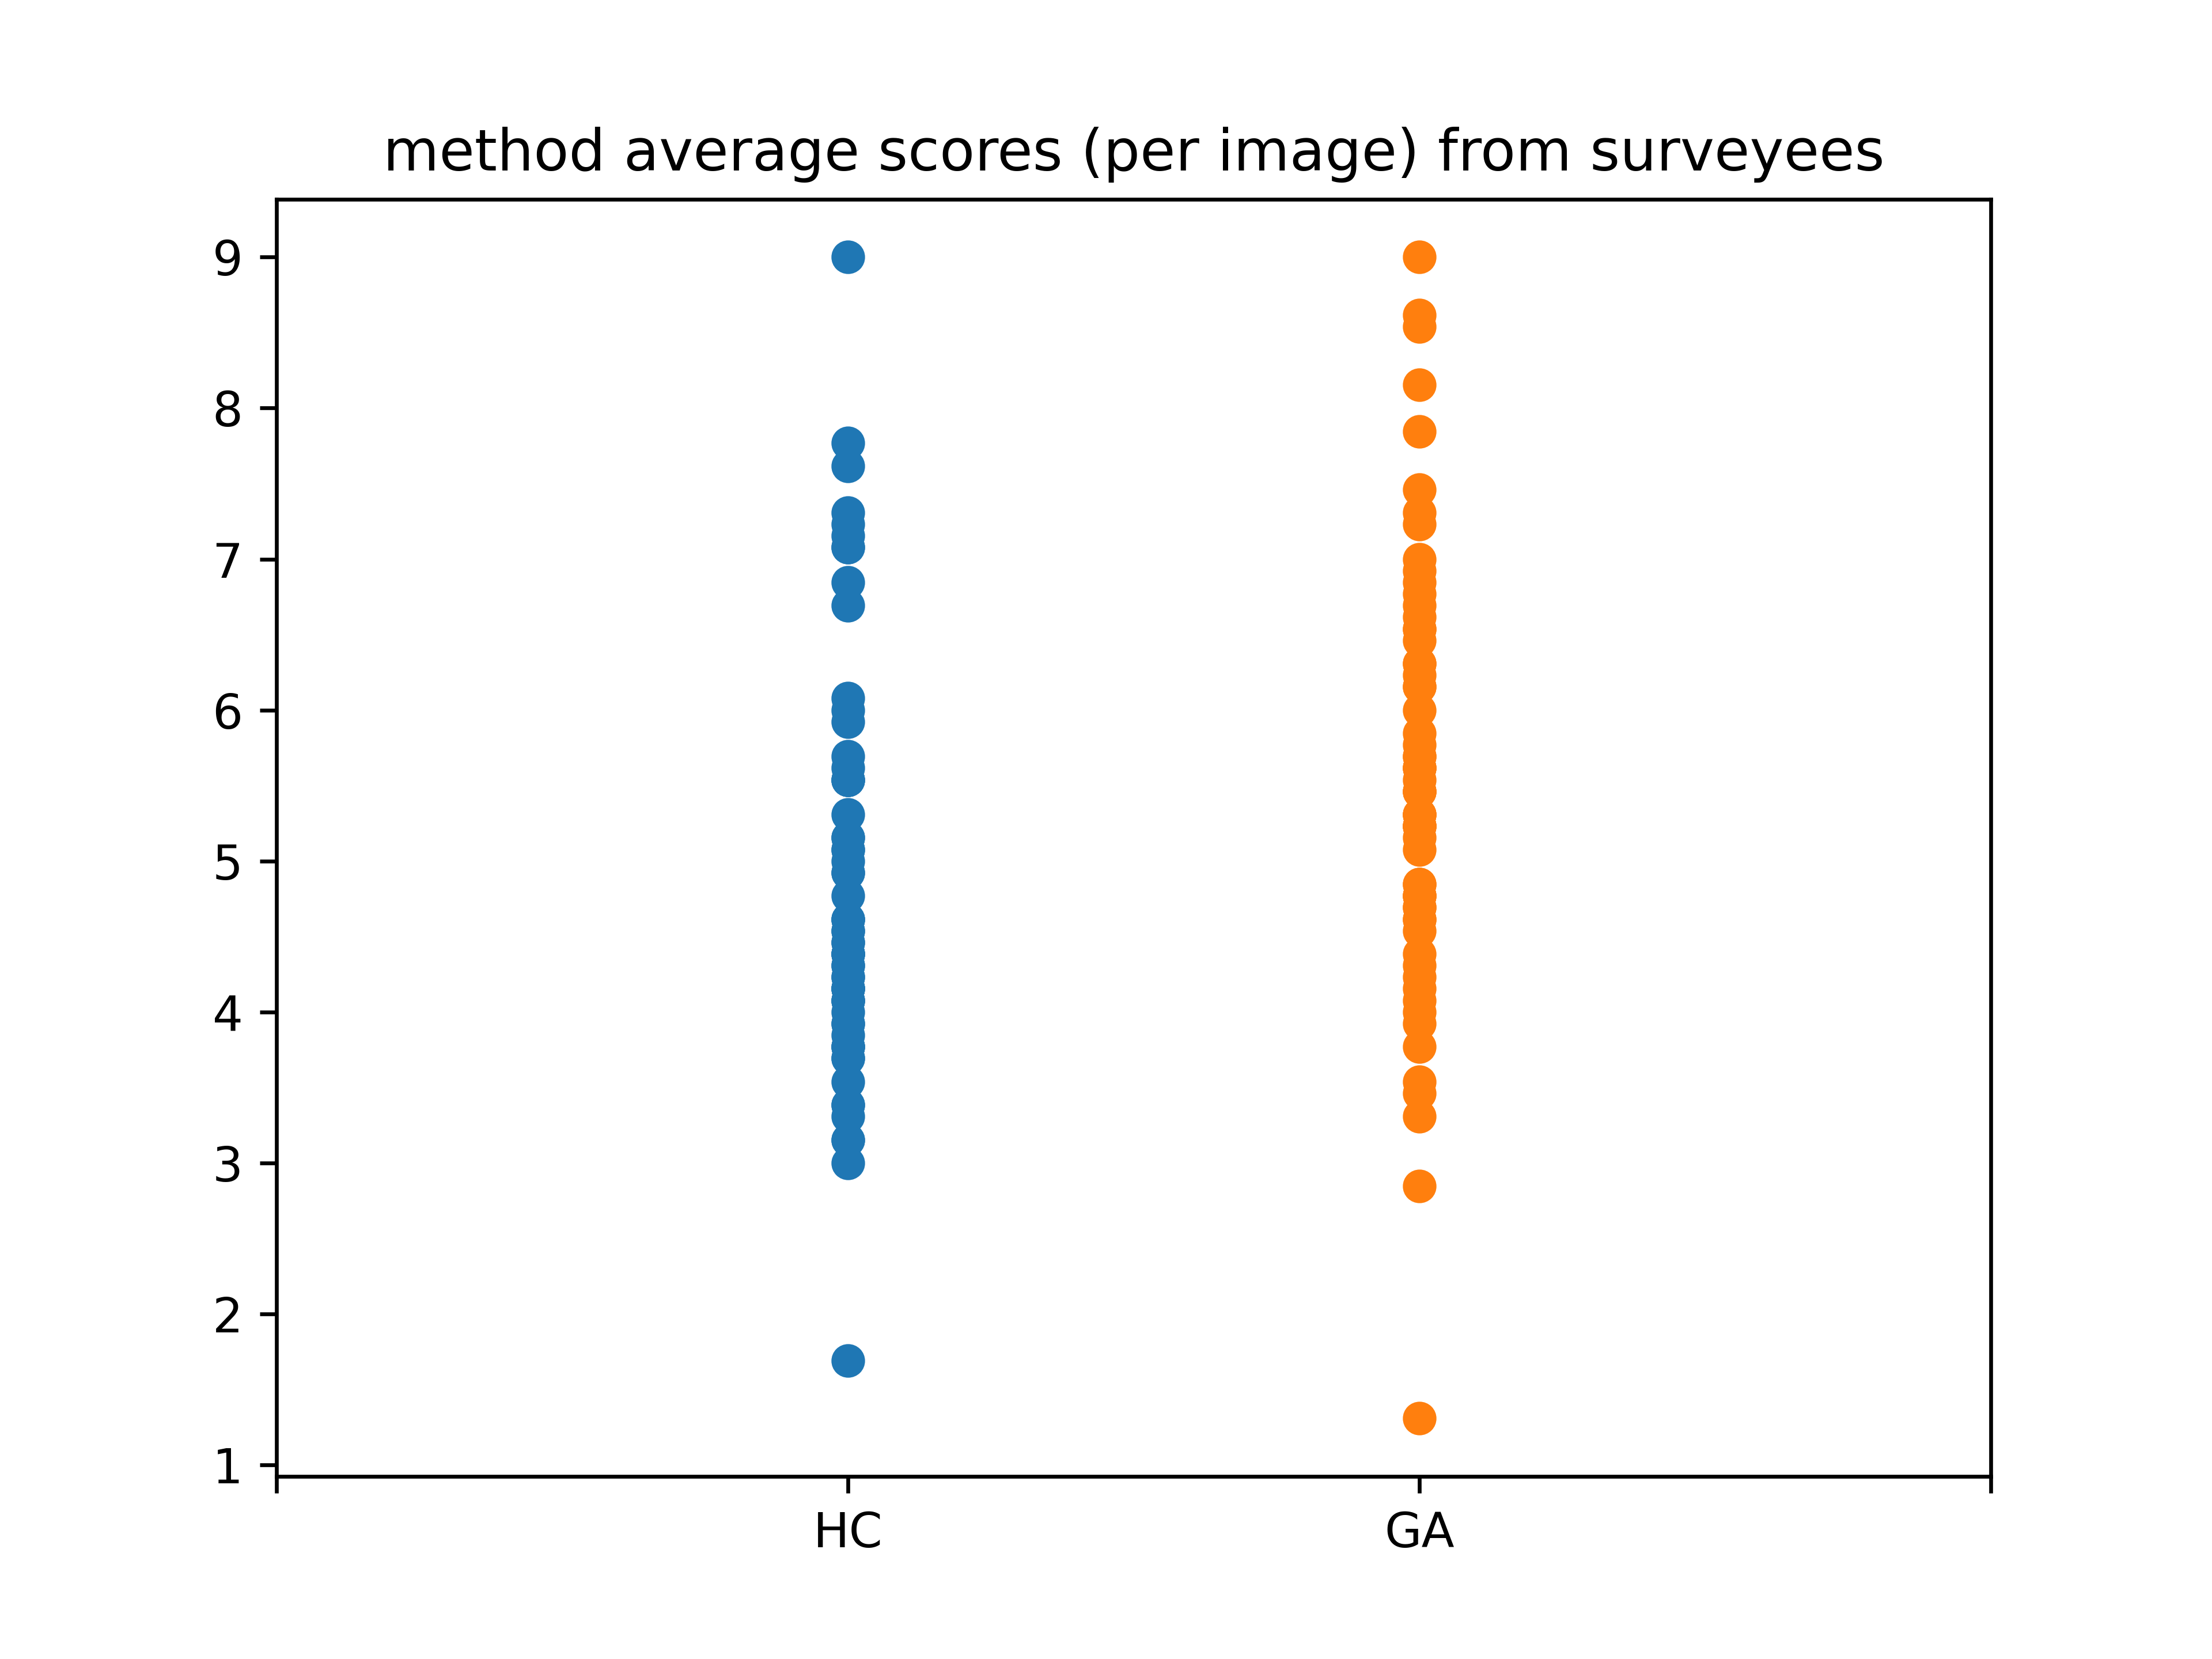
\includegraphics[width=\linewidth]{surveyee_score_scatter_plot.png}
  \caption{}
  \label{fig:survey_result_scatterplot}
\end{subfigure}
  \caption{Box plot of achieved score from survey participants of two methods. Method $1$ represents Hill Climbing with neighborhood generation with split mutation (\ref{subsubsection:method_hc_traptri_split}) and method $2$ represents Genetic Algorithm with (P, P) strategy (see Section \ref{subsection:method_ga_join}) }
  \label{fig:survey_result}
\end{figure}

From Figure \ref{fig:survey_result}, we can see the mean scores of all enhanced images given by each surveyee. 
Each data point in Figure \ref{fig:survey_result}(b) indicates the mean of scores given by one participant. Figure \ref{fig:survey_result}(a) shows the mean (triangle inside each box, green in color picture), and median (horizontal line inside each box, orange in color picture) of the responses. The red points are outliers according to the $1.5 \times$IQR rule \cite{rousseeuw2011robust}.

From Figure \ref{fig:survey_result}(a), method $2$ shows a better mean score than method $1$'s mean score (mean over participants). From Figure \ref{fig:survey_result}(b), we can see that method $1$ has a higher chance of degrading the image (dense below score $5$), although method $2$ has achieved the image with the lowest score according to one participant.

\begin{figure*}
  % one image
  \begin{subfigure}[b]{0.33\textwidth}%
    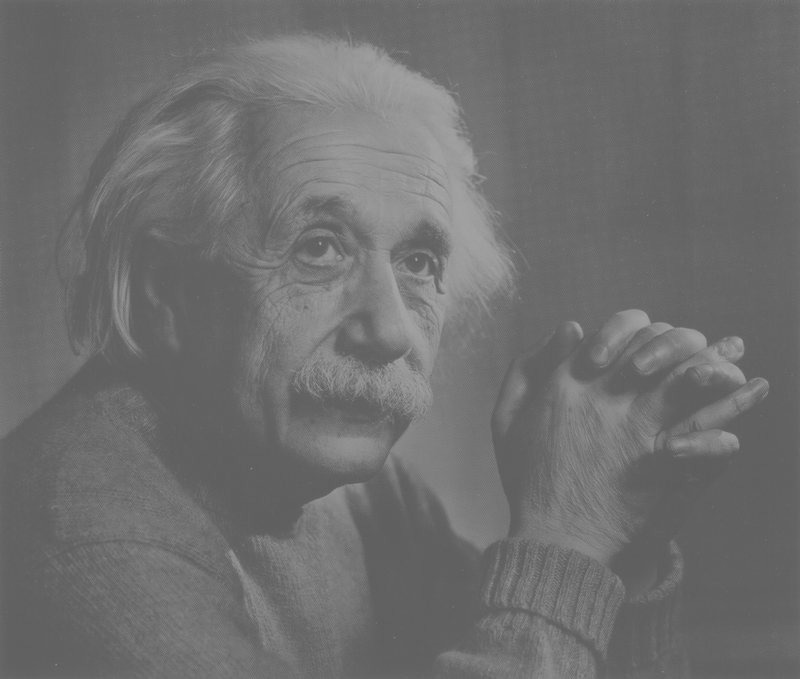
\includegraphics[width=\linewidth]{figures/original/07.jpg}
    \subcaption[]{}{}
    \label{fig:07_image_original}
  \end{subfigure}
  \begin{subfigure}[b]{0.33\textwidth}%
    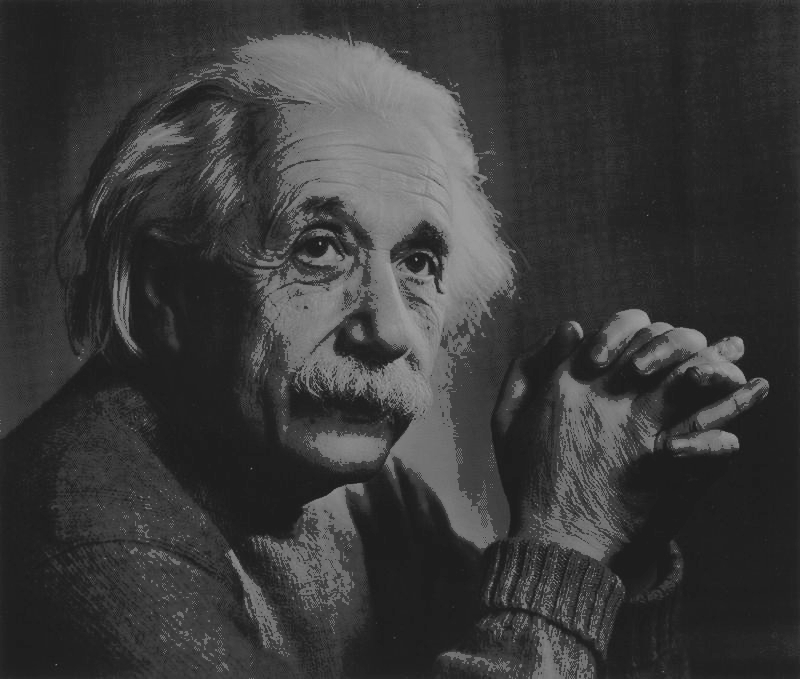
\includegraphics[width=\linewidth]{figures/hc_trap_split/07_output.jpg}
    \subcaption[]{}{}
    \label{fig:07_output_image_hc}
  \end{subfigure}
  \begin{subfigure}[b]{0.33\textwidth}%
    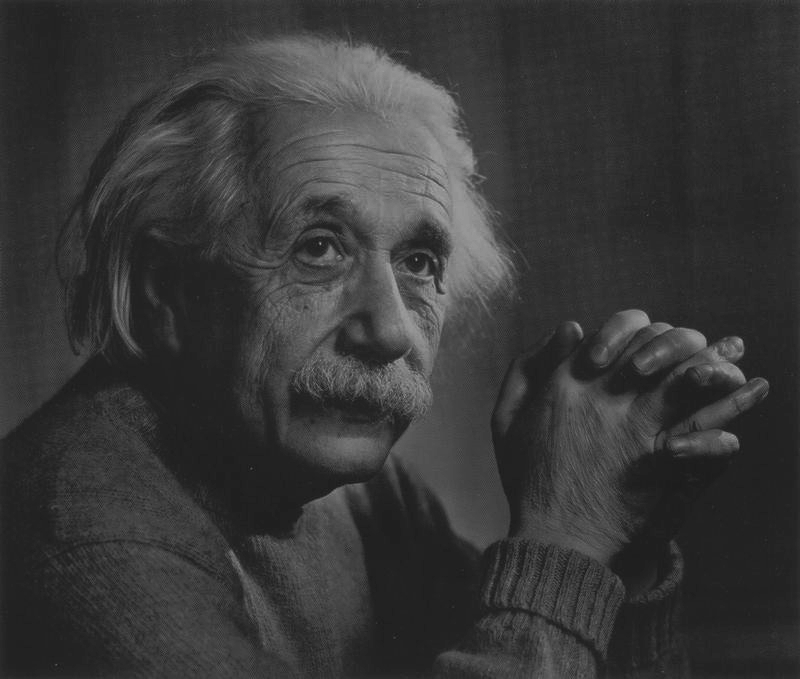
\includegraphics[width=\linewidth]{figures/ga_elitist/07_output.jpg}
    \subcaption[]{}{}
    \label{fig:07_output_image_ga}
  \end{subfigure}
  \vspace{-15pt}
  \caption{enhanced image generated by (b) simple HC (c) GA and (a) is original image}
  \label{fig:07_result}

  % one image
  \begin{subfigure}[b]{0.33\textwidth}
    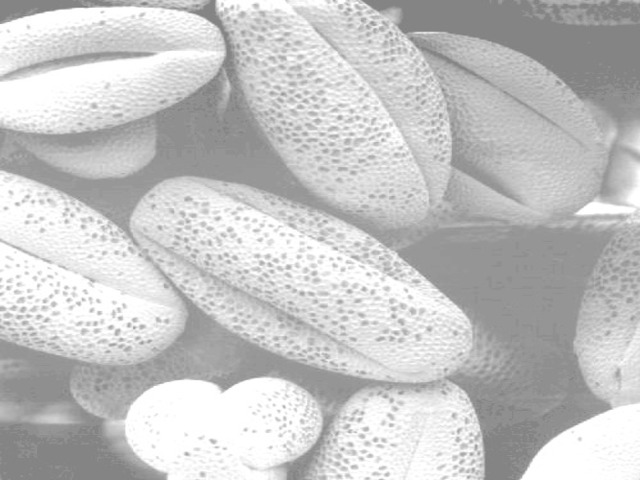
\includegraphics[width=\linewidth]{figures/original/08.jpg}
    \subcaption[]{}{}
    \label{fig:08_image_original}
  \end{subfigure}
  \begin{subfigure}[b]{0.33\textwidth}%
    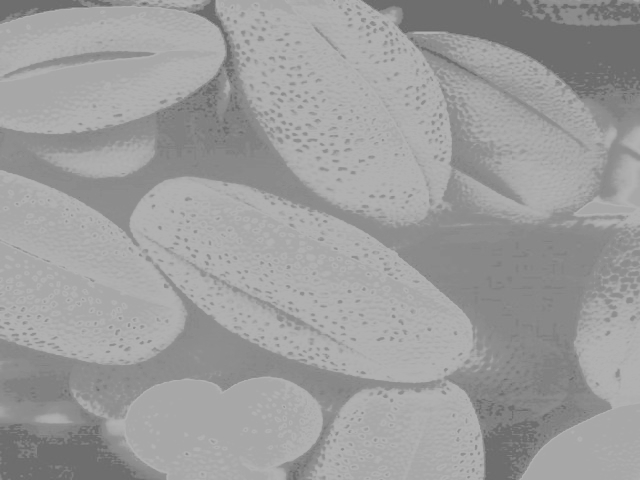
\includegraphics[width=\linewidth]{figures/hc_trap_split/08_output.jpg}
    \subcaption[]{}{}
    \label{fig:08_output_image_hc}
  \end{subfigure}
  \begin{subfigure}[b]{0.33\textwidth}%
    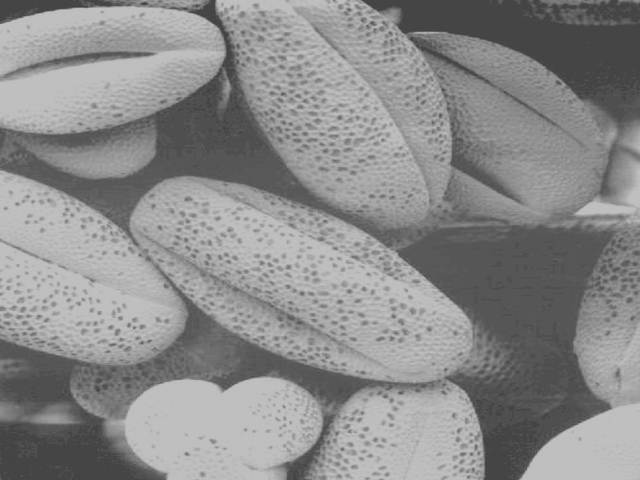
\includegraphics[width=\linewidth]{figures/ga_elitist/08_output.jpg}
    \subcaption[]{}{}
    \label{fig:08_output_image_ga}
  \end{subfigure}
  \vspace{-15pt}
  \caption{enhanced image generated by (b) simple HC (c) GA and (a) is original image}
  
  \label{fig:08_result}

  % one image
  \begin{subfigure}[b]{0.33\textwidth}
    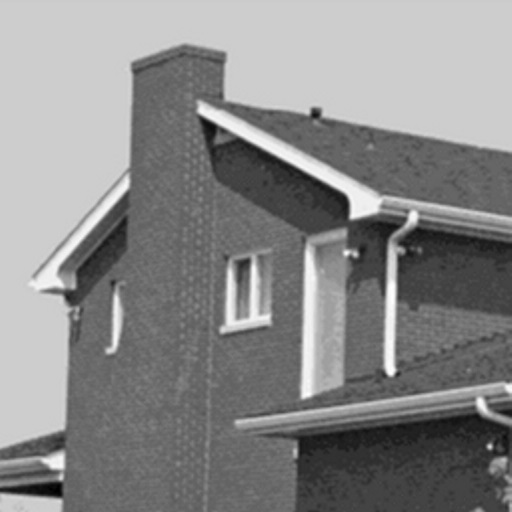
\includegraphics[width=\linewidth]{figures/original/house.jpg}
    \subcaption[]{}{}
    \label{fig:house_image_original}
  \end{subfigure}
  \begin{subfigure}[b]{0.33\textwidth}%
    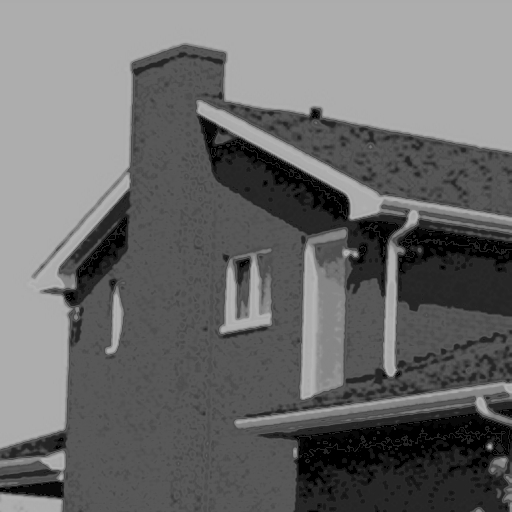
\includegraphics[width=\linewidth]{figures/hc_trap_split/house_output.jpg}
    \subcaption[]{}{}
    \label{fig:house_output_image_hc}
  \end{subfigure}
  \begin{subfigure}[b]{0.33\textwidth}%
    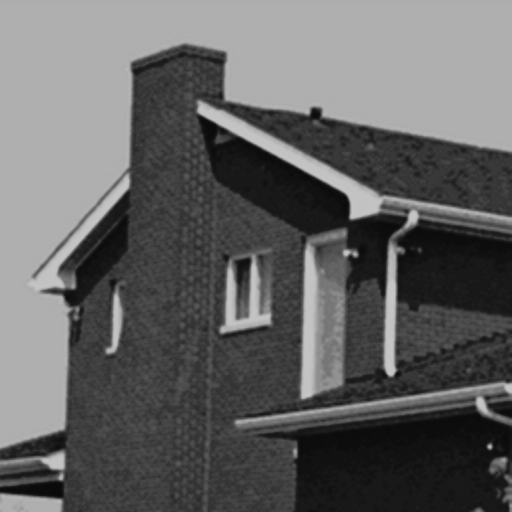
\includegraphics[width=\linewidth]{figures/ga_elitist/house_output.jpg}
    \subcaption[]{}{}
    \label{fig:house_output_image_ga}
  \end{subfigure}
  \vspace{-15pt}
  \caption{enhanced image generated by (b) simple HC (c) GA and (a) is original image}
  \label{fig:house_result}

  % one image
  \begin{subfigure}[b]{0.33\textwidth}
    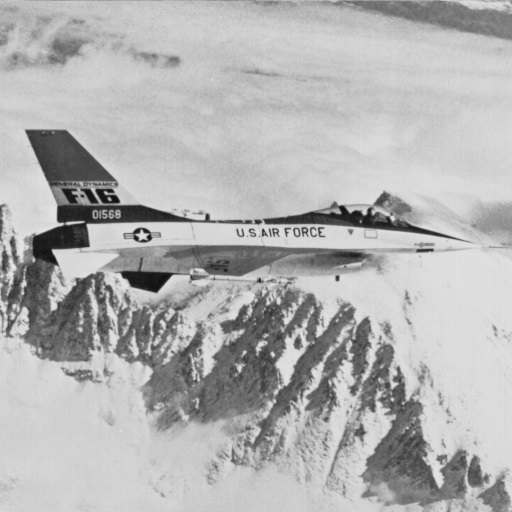
\includegraphics[width=\linewidth]{figures/original/jetplane.jpg}
    \subcaption[]{}{}
    \label{fig:jetplane_image_original}
  \end{subfigure}
  \begin{subfigure}[b]{0.33\textwidth}%
    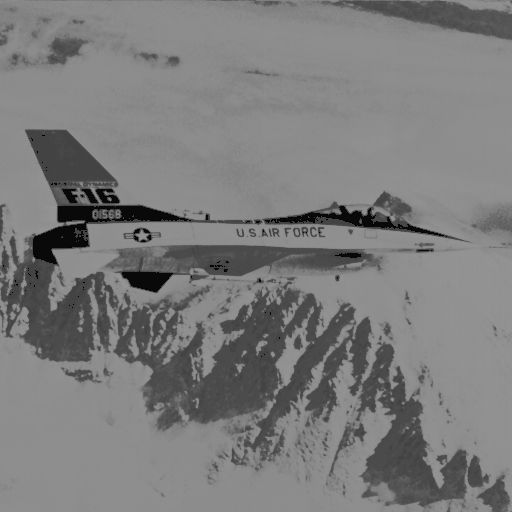
\includegraphics[width=\linewidth]{figures/hc_trap_split/jetplane_output.jpg}
    \subcaption[]{}{}
    \label{fig:jetplane_output_image_hc}
  \end{subfigure}
  \begin{subfigure}[b]{0.33\textwidth}%
    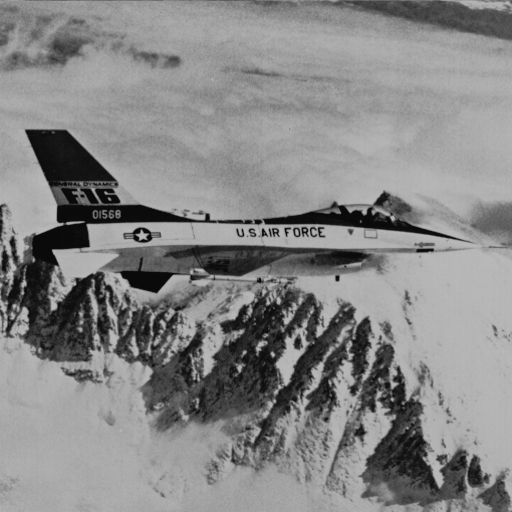
\includegraphics[width=\linewidth]{figures/ga_elitist/jetplane_output.jpg}
    \subcaption[]{}{}
    \label{fig:jetplane_output_image_ga}
  \end{subfigure}
  \vspace{-15pt}
  \caption{enhanced image generated by (b) simple HC (c) GA and (a) is original image}
  \label{fig:jetplane_result}
\end{figure*}

% next page
\begin{figure*}
  % one image
  \begin{subfigure}[b]{0.33\textwidth}
    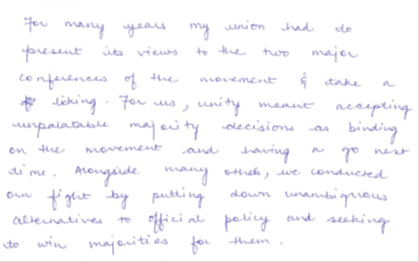
\includegraphics[width=\linewidth]{figures/original/11.png}
    \subcaption[]{}{}
    \label{fig:11_image_original}
  \end{subfigure}
  \begin{subfigure}[b]{0.33\textwidth}%
    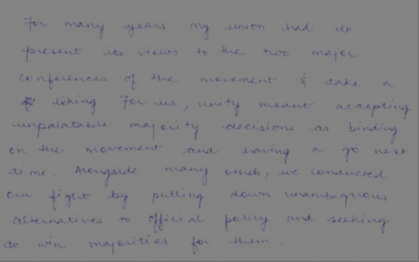
\includegraphics[width=\linewidth]{figures/hc_trap_split/11_output.jpg}
    \subcaption[]{}{}
    \label{fig:11_output_image_hc}
  \end{subfigure}
  \begin{subfigure}[b]{0.33\textwidth}%
    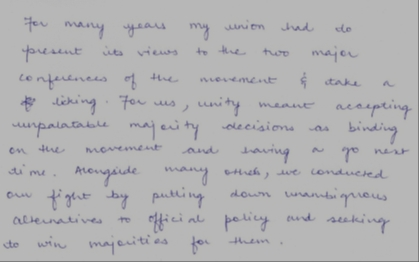
\includegraphics[width=\linewidth]{figures/ga_elitist/11_output.jpg}
    \subcaption[]{}{}
    \label{fig:11_output_image_ga}
  \end{subfigure}
  \caption{enhanced image generated by (b) simple HC (c) GA and (a) is original image}
  \label{fig:11_result}

  % one image
  \begin{subfigure}[b]{0.33\textwidth}
    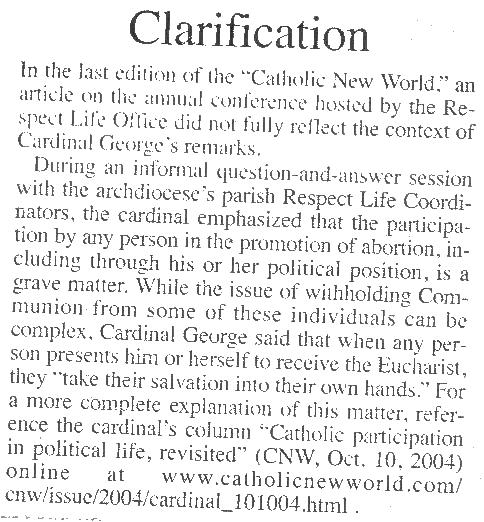
\includegraphics[width=\linewidth]{figures/original/12.jpg}
    \subcaption[]{}{}
    \label{fig:12_image_original}
  \end{subfigure}
  \begin{subfigure}[b]{0.33\textwidth}%
    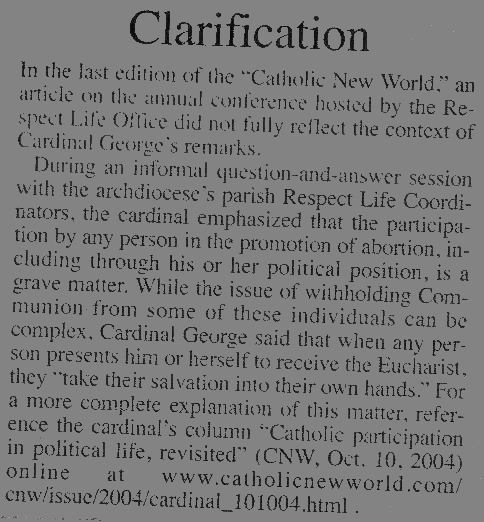
\includegraphics[width=\linewidth]{figures/hc_trap_split/12_output.jpg}
    \subcaption[]{}{}
    \label{fig:12_output_image_hc}
  \end{subfigure}
  \begin{subfigure}[b]{0.33\textwidth}%
    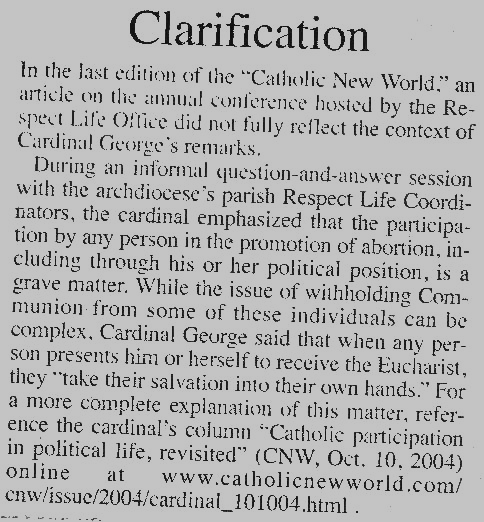
\includegraphics[width=\linewidth]{figures/ga_elitist/12_output.jpg}
    \subcaption[]{}{}
    \label{fig:12_output_image_ga}
  \end{subfigure}
  \caption{enhanced image generated by (b) simple HC (c) GA and (a) is original image}
  \label{fig:12_result}

  % one image
  \begin{subfigure}[b]{0.33\textwidth}
    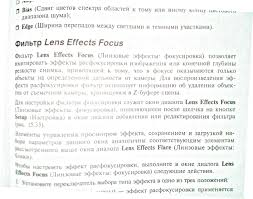
\includegraphics[width=\linewidth]{figures/original/13.jpg}
    \subcaption[]{}{}
    \label{fig:13_image_original}
  \end{subfigure}
  \begin{subfigure}[b]{0.33\textwidth}%
    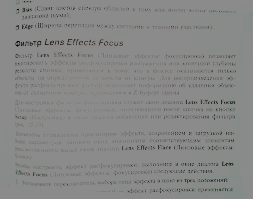
\includegraphics[width=\linewidth]{figures/hc_trap_split/13_output.jpg}
    \subcaption[]{}{}
    \label{fig:13_output_image_hc}
  \end{subfigure}
  \begin{subfigure}[b]{0.33\textwidth}%
    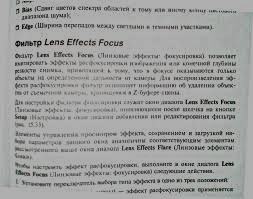
\includegraphics[width=\linewidth]{figures/ga_elitist/13_output.jpg}
    \subcaption[]{}{}
    \label{fig:13_output_image_ga}
  \end{subfigure}
  \caption{enhanced image generated by (b) simple HC (c) GA and (a) is original image}
  \label{fig:13_result}

  % one image
  \begin{subfigure}[b]{0.33\textwidth}
    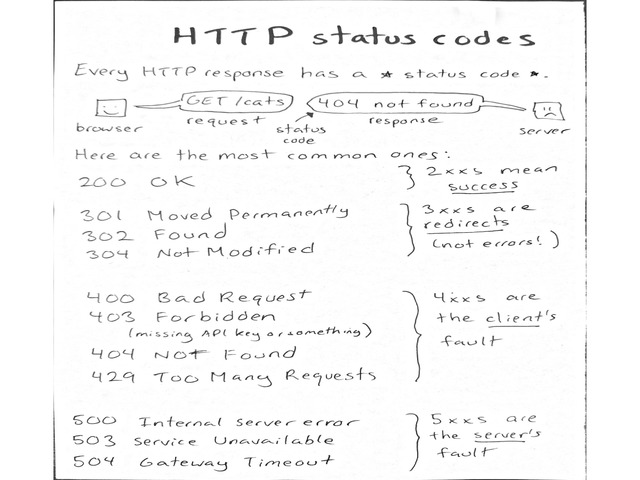
\includegraphics[width=\linewidth]{figures/original/09.jpg}
    \subcaption[]{}{}
    \label{fig:09_image_original}
  \end{subfigure}
  \begin{subfigure}[b]{0.33\textwidth}%
    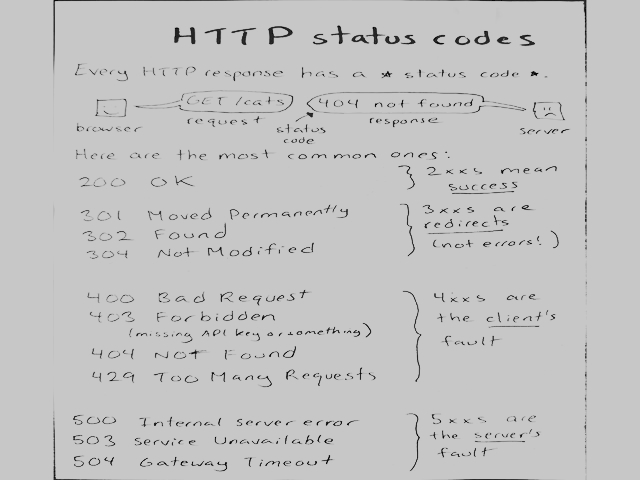
\includegraphics[width=\linewidth]{figures/hc_trap_split/09_output.jpg}
    \subcaption[]{}{}
    \label{fig:09_output_image_hc}
  \end{subfigure}
  \begin{subfigure}[b]{0.33\textwidth}%
    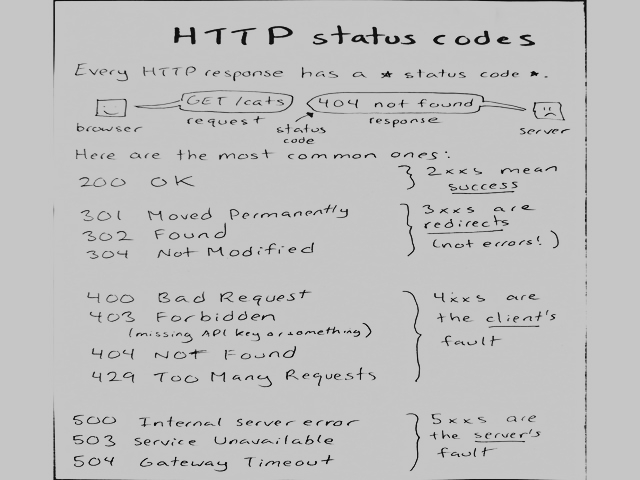
\includegraphics[width=\linewidth]{figures/ga_elitist/09_output.jpg}
    \subcaption[]{}{}
    \label{fig:09_output_image_ga}
  \end{subfigure}
  \caption{enhanced image generated by (b) simple HC (c) GA and (a) is original image}
  \label{fig:09_result}
\end{figure*}

% next page
\begin{figure*}
  % one image
  \begin{subfigure}[b]{0.33\textwidth}
    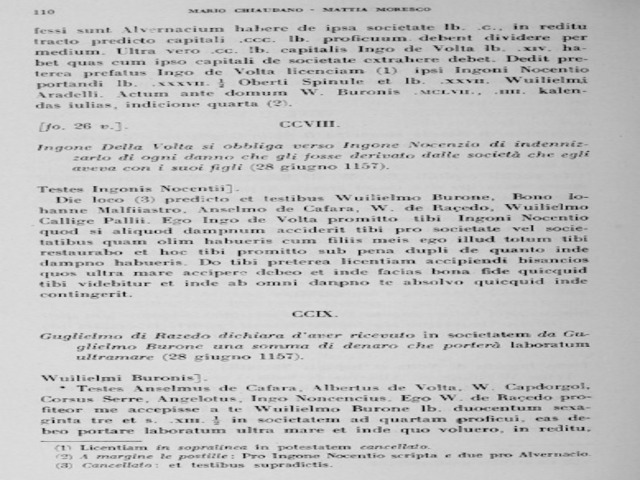
\includegraphics[width=\linewidth]{figures/original/10.jpg}
    \subcaption[]{}{}
    \label{fig:10_image_original}
  \end{subfigure}
  \begin{subfigure}[b]{0.33\textwidth}%
    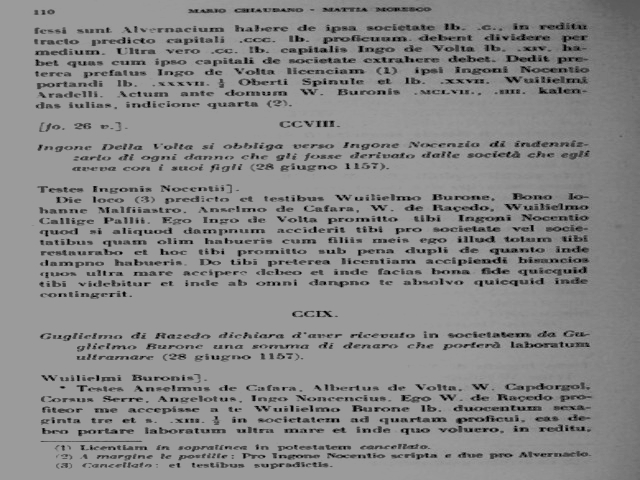
\includegraphics[width=\linewidth]{figures/hc_trap_split/10_output.jpg}
    \subcaption[]{}{}
    \label{fig:10_output_image_hc}
  \end{subfigure}
  \begin{subfigure}[b]{0.33\textwidth}%
    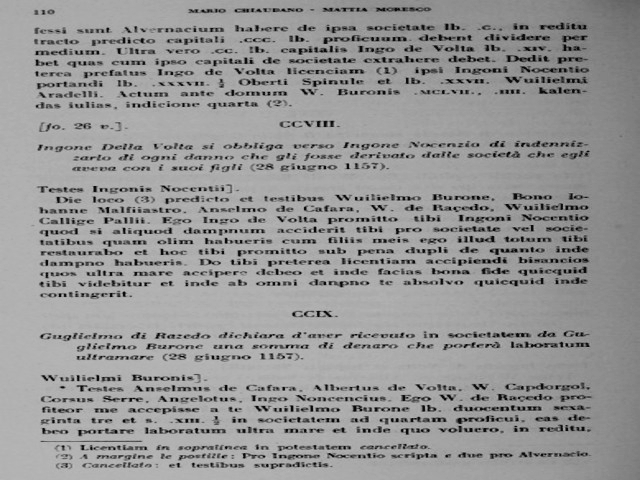
\includegraphics[width=\linewidth]{figures/ga_elitist/10_output.jpg}
    \subcaption[]{}{}
    \label{fig:10_output_image_ga}
  \end{subfigure}
  \caption{enhanced image generated by (b) simple HC (c) GA and (a) is original image}
  \label{fig:10_result}

  % one image
  \begin{subfigure}[b]{0.33\textwidth}
    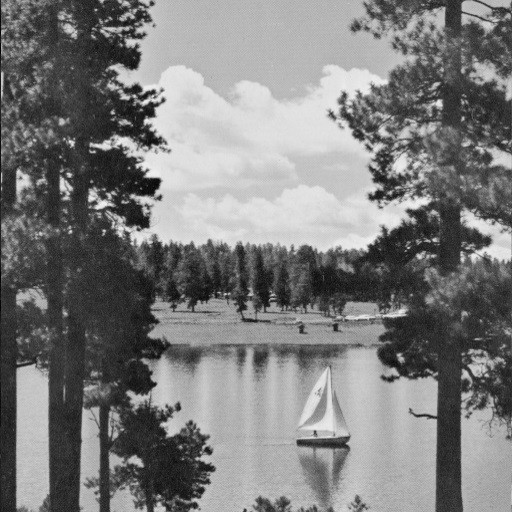
\includegraphics[width=\linewidth]{figures/original/lake.jpg}
    \subcaption[]{}{}
    \label{fig:lake_image_original}
  \end{subfigure}
  \begin{subfigure}[b]{0.33\textwidth}%
    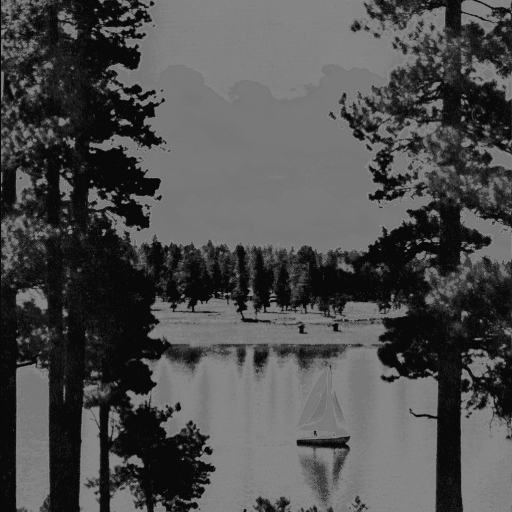
\includegraphics[width=\linewidth]{figures/hc_trap_split/lake_output.jpg}
    \subcaption[]{}{}
    \label{fig:lake_output_image_hc}
  \end{subfigure}
  \begin{subfigure}[b]{0.33\textwidth}%
    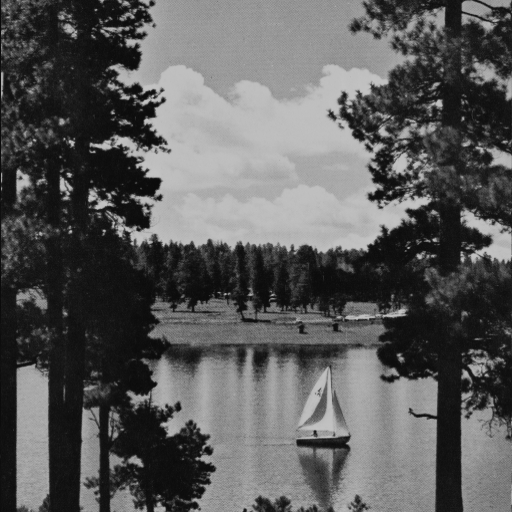
\includegraphics[width=\linewidth]{figures/ga_elitist/lake_output.jpg}
    \subcaption[]{}{}
    \label{fig:lake_output_image_ga}
  \end{subfigure}
  \caption{enhanced image generated by (b) simple HC (c) GA and (a) is original image}
  \label{fig:lake_result}

  % one image
  \begin{subfigure}[b]{0.33\textwidth}
    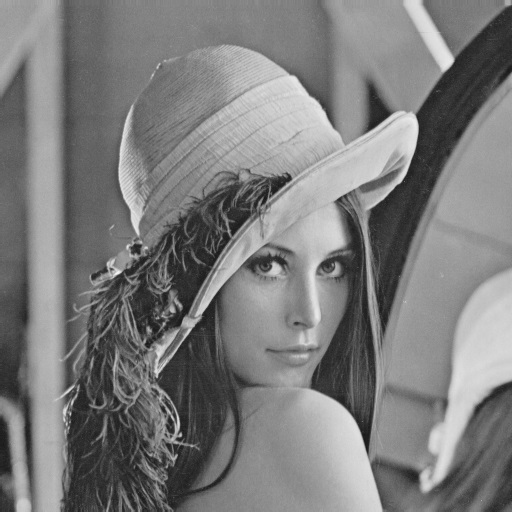
\includegraphics[width=\linewidth]{figures/original/lena_gray_512.jpg}
    \subcaption[]{}{}
    \label{fig:lenagray_image_original}
  \end{subfigure}
  \begin{subfigure}[b]{0.33\textwidth}%
    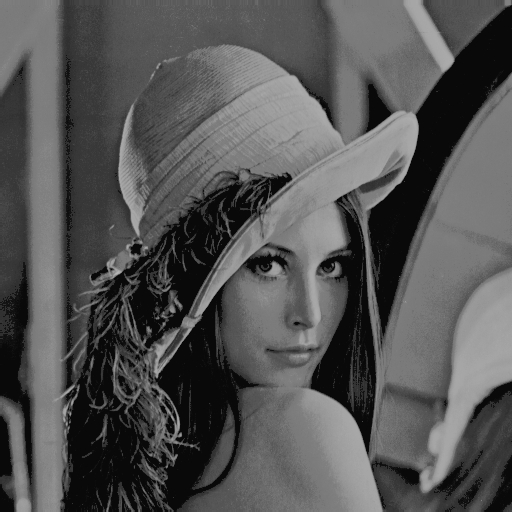
\includegraphics[width=\linewidth]{figures/hc_trap_split/lena_gray_512_output.jpg}
    \subcaption[]{}{}
    \label{fig:lenagray_output_image_hc}
  \end{subfigure}
  \begin{subfigure}[b]{0.33\textwidth}%
    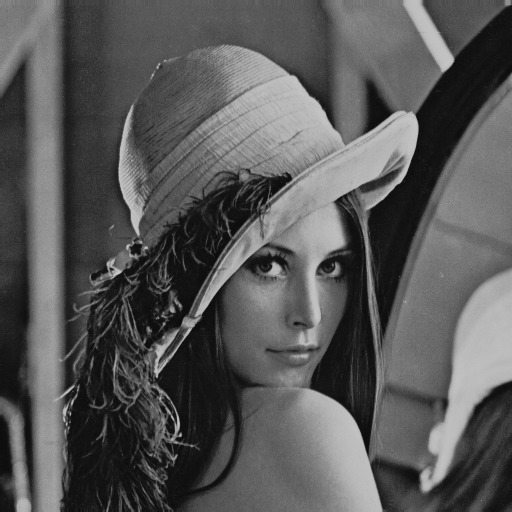
\includegraphics[width=\linewidth]{figures/ga_elitist/lena_gray_512_output.jpg}
    \subcaption[]{}{}
    \label{fig:lenagray_output_image_ga}
  \end{subfigure}
  \caption{enhanced image generated by (b) simple HC (c) GA and (a) is original image}
  \label{fig:lenagray_result}
\end{figure*}

% next page
\begin{figure*}
  % one image
  \begin{subfigure}[b]{0.33\textwidth}
    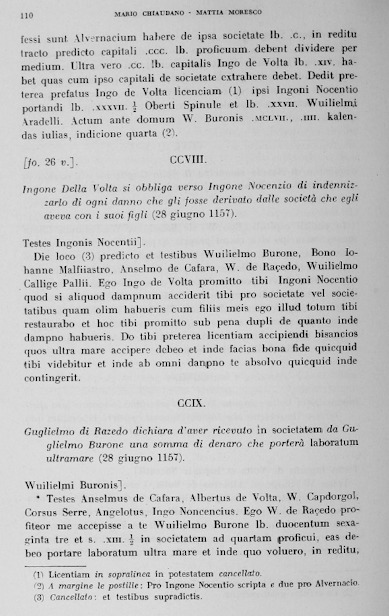
\includegraphics[width=\linewidth]{figures/original/06.jpg}
    \subcaption[]{}{}
    \label{fig:06_image_original}
  \end{subfigure}
  \begin{subfigure}[b]{0.33\textwidth}%
    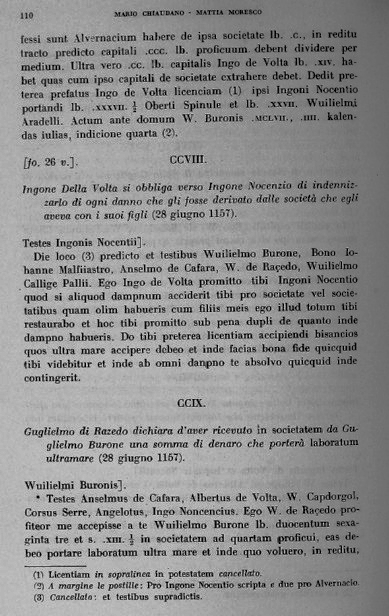
\includegraphics[width=\linewidth]{figures/hc_trap_split/06_output.jpg}
    \subcaption[]{}{}
    \label{fig:06_output_image_hc}
  \end{subfigure}
  \begin{subfigure}[b]{0.33\textwidth}%
    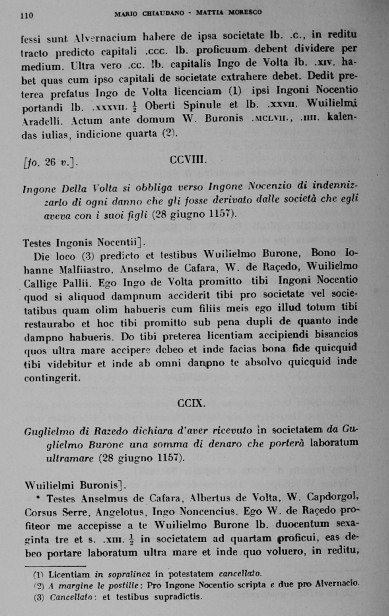
\includegraphics[width=\linewidth]{figures/ga_elitist/06_output.jpg}
    \subcaption[]{}{}
    \label{fig:06_output_image_ga}
  \end{subfigure}
  \caption{enhanced image generated by (b) simple HC (c) GA and (a) is original image}
  \label{fig:06_result}

  % one image
  \begin{subfigure}[b]{0.33\textwidth}
    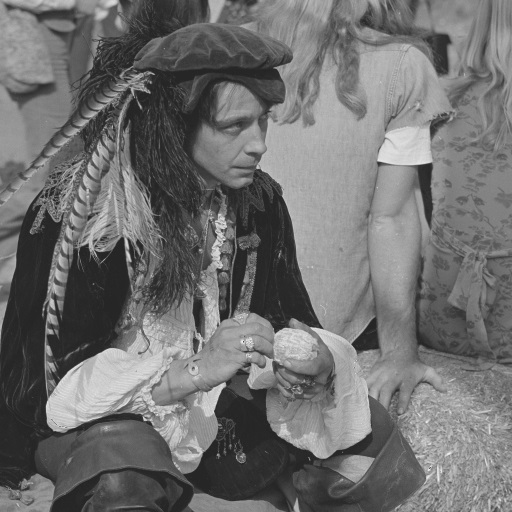
\includegraphics[width=\linewidth]{figures/original/pirate.jpg}
    \subcaption[]{}{}
    \label{fig:pirate_image_original}
  \end{subfigure}
  \begin{subfigure}[b]{0.33\textwidth}%
    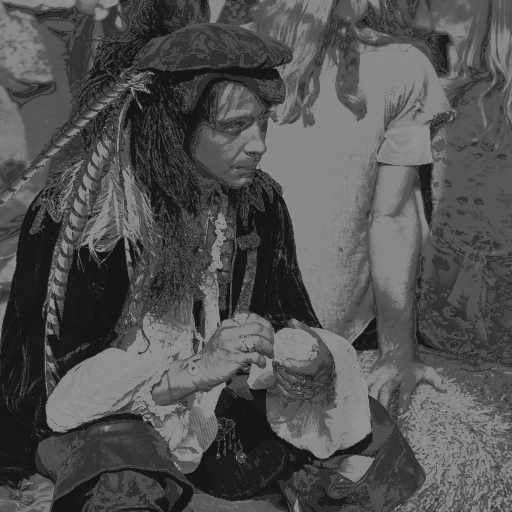
\includegraphics[width=\linewidth]{figures/hc_trap_split/pirate_output.jpg}
    \subcaption[]{}{}
    \label{fig:pirate_output_image_hc}
  \end{subfigure}
  \begin{subfigure}[b]{0.33\textwidth}%
    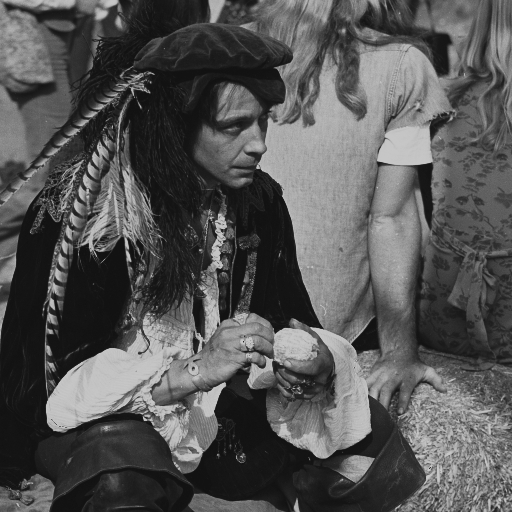
\includegraphics[width=\linewidth]{figures/ga_elitist/pirate_output.jpg}
    \subcaption[]{}{}
    \label{fig:pirate_output_image_ga}
  \end{subfigure}
  \caption{enhanced image generated by (b) simple HC (c) GA and (a) is original image}
  \label{fig:pirate_result}
\end{figure*}
\section{Conclusion}
We have applied meta-heuristics to find a good image-specific fuzzy logic-based transformation function in this work. We have employed a quality function from some previous works. As image quality is subjective, to assess our method's success, we have conducted a survey to gain subjective opinions on the visual quality of enhancement and reported the result. From the assessment, we have seen that one variant among the five gives us a visual improvement on average.

For future work, more experiments can be done by associating more image processing operations (e.g., gamma transformation) can be added in the processing pipeline. One limitation of our approach (according to visual observation) is that it darkens the image. Adding other processing operations with automatic parameter tuning through meta-heuristics seems promising for further improvement.

\iffalse
\paragraph{Sample Heading (Fourth Level)}
The contribution should contain no more than four levels of
headings. Table~\ref{tab1} gives a summary of all heading levels.

\begin{table}
\caption{Table captions should be placed above the
tables.}\label{tab1}
\begin{tabular}{|l|l|l|}
\hline
Heading level &  Example & Font size and style\\
\hline
Title (centered) &  {\Large\bfseries Lecture Notes} & 14 point, bold\\
1st-level heading &  {\large\bfseries 1 Introduction} & 12 point, bold\\
2nd-level heading & {\bfseries 2.1 Printing Area} & 10 point, bold\\
3rd-level heading & {\bfseries Run-in Heading in Bold.} Text follows & 10 point, bold\\
4th-level heading & {\itshape Lowest Level Heading.} Text follows & 10 point, italic\\
\hline
\end{tabular}
\end{table}


\noindent Displayed equations are centered and set on a separate
line.
\begin{equation}
x + y = z
\end{equation}
Please try to avoid rasterized images for line-art diagrams and
schemas. Whenever possible, use vector graphics instead (see
Fig.~\ref{fig1}).

\begin{figure}
\includegraphics[width=\textwidth]{fig1.eps}
\caption{A figure caption is always placed below the illustration.
Please note that short captions are centered, while long ones are
justified by the macro package automatically.} \label{fig1}
\end{figure}

\begin{theorem}
This is a sample theorem. The run-in heading is set in bold, while
the following text appears in italics. Definitions, lemmas,
propositions, and corollaries are styled the same way.
\end{theorem}
%
% the environments 'definition', 'lemma', 'proposition', 'corollary',
% 'remark', and 'example' are defined in the LLNCS documentclass as well.
%
\begin{proof}
Proofs, examples, and remarks have the initial word in italics,
while the following text appears in normal font.
\end{proof}
For citations of references, we prefer the use of square brackets
and consecutive numbers. Citations using labels or the author/year
convention are also acceptable. The following bibliography provides
a sample reference list with entries for journal
articles~\cite{ref_article1}, an LNCS chapter~\cite{ref_lncs1}, a
book~\cite{ref_book1}, proceedings without editors~\cite{ref_proc1},
and a homepage~\cite{ref_url1}. Multiple citations are grouped
\cite{ref_article1,ref_lncs1,ref_book1},
\cite{ref_article1,ref_book1,ref_proc1,ref_url1}.
\fi
%
% ---- Bibliography ----
%
% BibTeX users should specify bibliography style 'splncs04'.
% References will then be sorted and formatted in the correct style.
%
% \bibliographystyle{named}
% \bibliography{mybibliography}

% \section*{Code and Data Availability}
% The code and data can be found at the following link: \href{https://dicta2024.dictaconference.org}{redacted for review version}%\url{ https://bitbucket.org/mahi045/image-enhancement/src/master/}

% \section*{Conflict of Interest}
% The authors declare no conflict of interest.

\bibliographystyle{IEEEtran}
\bibliography{main}
% \begin{thebibliography}{00}
% \bibitem{cuckoo_search_and_PSO}
% Ye, Zhiwei, Mingwei Wang, Zhengbing Hu, and Wei Liu. "An adaptive image enhancement technique by combining cuckoo search and particle swarm optimization algorithm." Computational intelligence and neuroscience 2015 (2015).

% \bibitem{ACO_GA_SA}
% Hoseini, Pourya, and Mahrokh G. Shayesteh. "Efficient contrast enhancement of images using hybrid ant colony optimisation, genetic algorithm, and simulated annealing." Digital Signal Processing 23.3 (2013): 879-893.

% \bibitem{draa2014artificial}
% A. Draa and A. Bouaziz. (2014). An artificial bee colony algorithm for image contrast enhancement. Swarm and Evolutionary Computation. 16. 10.1016/j.swevo.2014.01.003. 
% \bibitem{hashemi2010image} Sara Hashemi, Soheila Kiani, Navid Noroozi, and Mohsen Ebrahimi Moghaddam. 2010. An image contrast enhancement method based on genetic algorithm. Pattern Recogn. Lett. 31, 13 (October 2010), 1816–1824. 

% \bibitem{fuzzy_plus_meta}
% Fernandez, Alberto, Victoria Lopez, Maria Jose del Jesus, and Francisco Herrera. "Revisiting evolutionary fuzzy systems: Taxonomy, applications, new trends and challenges." Knowledge-Based Systems 80 (2015): 109-121.
  

% \bibitem{gonzalez2008digital} Rafael C. Gonzalez and Richard E. Woods. 2006. Digital Image Processing (3rd Edition). Prentice-Hall, Inc., USA.
% \bibitem{Luke2009Metaheuristics} Sean Luke, 2013, Essentials of Metaheuristics, Lulu, second edition.
% \bibitem{stark2000adaptive} J. A. Stark, "Adaptive image contrast enhancement using generalizations of histogram equalization," in IEEE Transactions on Image Processing, vol. 9, no. 5, pp. 889-896, May 2000.
% doi: 10.1109/83.841534
% \bibitem{shanmugavadivu2014particle} P. Shanmugavadivu, K. Balasubramanian,
% Particle swarm optimized multi-objective histogram equalization for image enhancement,
% Optics \& Laser Technology, Volume 57, 2014,
% Pages 243-251,
% ISSN 0030-3992,
% \url{https://doi.org/10.1016/j.optlastec.2013.07.013}.
% \bibitem{oloyede2019new} Oloyede, M., Hancke, G., Myburgh, H. et al. A new evaluation function for face image enhancement in unconstrained environments using metaheuristic algorithms. J Image Video Proc. 2019, 27 (2019).\url{https://doi.org/10.1186/s13640-019-0418-7}
% \bibitem{zhu2012adaptive} Youlian Zhu, Cheng Huang,
% An Adaptive Histogram Equalization Algorithm on the Image Gray Level Mapping,
% Physics Procedia,
% Volume 25,
% 2012,
% Pages 601-608,
% ISSN 1875-3892,
% \url{https://doi.org/10.1016/j.phpro.2012.03.132}.
% \bibitem{s2018image}
% Joshi, Sandeep \& Kumar, Samrudh. (2018). Image contrast enhancement using fuzzy logic. 
% \bibitem{munteanu2004gray}
% C. Munteanu and A. Rosa, "Gray-scale image enhancement as an automatic process driven by evolution," in IEEE Transactions on Systems, Man, and Cybernetics, Part B (Cybernetics), vol. 34, no. 2, pp. 1292-1298, April 2004.
% doi: 10.1109/TSMCB.2003.818533
% \bibitem{samanta2018log}
% Samanta, Sourav \& Mukherjee, Amartya \& Ashour, Amira S. \& Dey, Nilanjan \& Tavares, Joao \& ABDESSALEMKARAA, WAHIBA \& Taiar, Redha \& Azar, Ahmad \& Hassanien, Aboul Ella. (2018). Log Transform Based Optimal Image Enhancement Using Firefly Algorithm for Autonomous Mini Unmanned Aerial Vehicle: An Application of Aerial Photography. International Journal of Image and Graphics. 18. 1850019. 10.1142/S0219467818500195. 
% \bibitem{bhandari2019cuckoo}
% Bhandari, A. \& Maurya, Shubham. (2019). Cuckoo search algorithm-based brightness preserving histogram scheme for low-contrast image enhancement. Soft Computing. 10.1007/s00500-019-03992-7. 
% \bibitem{dos2009differential}
% Coelho, Leandro \& Sauer, João \& Rudek, Marcelo. (2009). Differential evolution optimization combined with chaotic sequences for image contrast enhancement. Chaos, Solitons \& Fractals. 42. 522-529. 10.1016/j.chaos.2009.01.012. 
% \bibitem{braik2007particle}
% Braik, Malik \& Sheta, Alaa \& Ayesh, Aladdin. (2007). Particle swarm optimisation enhancement approach for improving image quality. International Journal of Innovative Computing and Applications. 1. 10.1504/IJICA.2007.016795. 
% \bibitem{unknown}
% Joshi, Sandeep \& Kumar, Samrudh. (2018). Image contrast enhancement using fuzzy logic. 
% \bibitem{Fuzzy}
% Haußecker, Horst \& Tizhoosh, Hamid. (1999). Fuzzy Image Processing. 10.1016/B978-012379777-3/50017-0. 

% \bibitem{gamma}
% A. S. Tarawneh, A. B. Hassanat, I. Elkhadiri, D. Chetverikov and K. Almohammadi, "Automatic Gamma Correction Based on Root-Mean-Square-Error Maximization," 2020 International Conference on Computing and Information Technology (ICCIT-1441), 2020, pp. 1-5, doi: 10.1109/ICCIT-144147971.2020.9213752.

% \bibitem{iqr}
% Rousseeuw, P.J. and Hubert, M., 2011. Robust statistics for outlier detection. Wiley interdisciplinary reviews: Data mining and knowledge discovery, 1(1), pp.73-79.

% \bibitem{guan2009image}
% Singh, G., \& Mittal, A. (2014). Various image enhancement techniques-a critical review. International Journal of Innovation and Scientific Research, 10(2), 267-274.
% \bibitem{singh2015histogram}
% Singh, Ravindra Pal, and Manish Dixit. "Histogram equalization: a strong technique for image enhancement." International Journal of Signal Processing, Image Processing and Pattern Recognition 8, no. 8 (2015): 345-352.

% \bibitem{ooi2009bi}
% Ooi, C. H., Kong, N. S. P., \& Ibrahim, H. (2009). Bi-histogram equalization with a plateau limit for digital image enhancement. IEEE transactions on consumer electronics, 55(4), 2072-2080.

% \bibitem{singh2014various}
% Singh, G., \& Mittal, A. (2014). Various image enhancement techniques-a critical review. International Journal of Innovation and Scientific Research, 10(2), 267-274.



% \end{thebibliography}
%
\end{document}
